% Options for packages loaded elsewhere
\PassOptionsToPackage{unicode}{hyperref}
\PassOptionsToPackage{hyphens}{url}
%
\documentclass[
  11pt,
  a4paper,
]{article}
\usepackage{amsmath,amssymb}
\usepackage{lmodern}
\usepackage{ifxetex,ifluatex}
\ifnum 0\ifxetex 1\fi\ifluatex 1\fi=0 % if pdftex
  \usepackage[T1]{fontenc}
  \usepackage[utf8]{inputenc}
  \usepackage{textcomp} % provide euro and other symbols
\else % if luatex or xetex
  \usepackage{unicode-math}
  \defaultfontfeatures{Scale=MatchLowercase}
  \defaultfontfeatures[\rmfamily]{Ligatures=TeX,Scale=1}
  \setmainfont[]{Times New Roman}
  \setsansfont[]{Times New Roman}
\fi
% Use upquote if available, for straight quotes in verbatim environments
\IfFileExists{upquote.sty}{\usepackage{upquote}}{}
\IfFileExists{microtype.sty}{% use microtype if available
  \usepackage[]{microtype}
  \UseMicrotypeSet[protrusion]{basicmath} % disable protrusion for tt fonts
}{}
\makeatletter
\@ifundefined{KOMAClassName}{% if non-KOMA class
  \IfFileExists{parskip.sty}{%
    \usepackage{parskip}
  }{% else
    \setlength{\parindent}{0pt}
    \setlength{\parskip}{6pt plus 2pt minus 1pt}}
}{% if KOMA class
  \KOMAoptions{parskip=half}}
\makeatother
\usepackage{xcolor}
\IfFileExists{xurl.sty}{\usepackage{xurl}}{} % add URL line breaks if available
\IfFileExists{bookmark.sty}{\usepackage{bookmark}}{\usepackage{hyperref}}
\hypersetup{
  pdftitle={Banco de Portugal's Microdata Research Laboratory},
  pdfauthor={BPLIM: External Server Manual},
  hidelinks,
  pdfcreator={LaTeX via pandoc}}
\urlstyle{same} % disable monospaced font for URLs
\usepackage{longtable,booktabs,array}
\usepackage{calc} % for calculating minipage widths
% Correct order of tables after \paragraph or \subparagraph
\usepackage{etoolbox}
\makeatletter
\patchcmd\longtable{\par}{\if@noskipsec\mbox{}\fi\par}{}{}
\makeatother
% Allow footnotes in longtable head/foot
\IfFileExists{footnotehyper.sty}{\usepackage{footnotehyper}}{\usepackage{footnote}}
\makesavenoteenv{longtable}
\usepackage{graphicx}
\makeatletter
\def\maxwidth{\ifdim\Gin@nat@width>\linewidth\linewidth\else\Gin@nat@width\fi}
\def\maxheight{\ifdim\Gin@nat@height>\textheight\textheight\else\Gin@nat@height\fi}
\makeatother
% Scale images if necessary, so that they will not overflow the page
% margins by default, and it is still possible to overwrite the defaults
% using explicit options in \includegraphics[width, height, ...]{}
\setkeys{Gin}{width=\maxwidth,height=\maxheight,keepaspectratio}
% Set default figure placement to htbp
\makeatletter
\def\fps@figure{htbp}
\makeatother
\usepackage[normalem]{ulem}
% Avoid problems with \sout in headers with hyperref
\pdfstringdefDisableCommands{\renewcommand{\sout}{}}
\setlength{\emergencystretch}{3em} % prevent overfull lines
\providecommand{\tightlist}{%
  \setlength{\itemsep}{0pt}\setlength{\parskip}{0pt}}
\setcounter{secnumdepth}{5}
\usepackage[paperwidth=210mm,paperheight=297mm,left=27mm,right=27mm,top=25mm,bottom=25mm]{geometry} \usepackage{hyperref} \hypersetup{colorlinks=true} \hypersetup{citecolor=black} \hypersetup{linkcolor=blue!75!black} \hypersetup{urlcolor=blue!75!black} \hypersetup{filecolor=blue!75!black} \hypersetup{citecolor=black} \usepackage{float} \usepackage{dcolumn} \usepackage{color} \usepackage{pdfpages} \usepackage{setspace} \doublespacing
\ifluatex
  \usepackage{selnolig}  % disable illegal ligatures
\fi

\title{Banco de Portugal's Microdata Research Laboratory}
\author{\href{https://bplim.bportugal.pt/}{BPLIM}: External Server
Manual}
\date{\texttt{r\ format(Sys.time(),\ \textquotesingle{}\%d\ \%B,\ \%Y\textquotesingle{})}}

\begin{document}
\maketitle

{
\setcounter{tocdepth}{2}
\tableofcontents
}
\newpage

\hypertarget{access-to-the-external-server}{%
\section{Access to the External
Server}\label{access-to-the-external-server}}

\hypertarget{upon-access-approval}{%
\subsection{Upon access approval}\label{upon-access-approval}}

The User will be able to connect to the external server using
\texttt{NoMachine} client access: see
\protect\hyperlink{install_nomachine}{Section 8.4} for details on
installation and use.

\hypertarget{password-policy}{%
\subsection{Password policy}\label{password-policy}}

\begin{itemize}
\tightlist
\item
  The first password delivered must be changed at the first login.
\item
  After \textbf{60 days} the password will expire: the login window will
  show \texttt{new\ password}
\item
  The passwords to be specified must meet the requirements described in
  \protect\hyperlink{password}{Section 8.3}.
\end{itemize}

\hypertarget{first-steps}{%
\subsection{First steps}\label{first-steps}}

Once you start \texttt{NoMachine}, these are the first three screens you
will see:

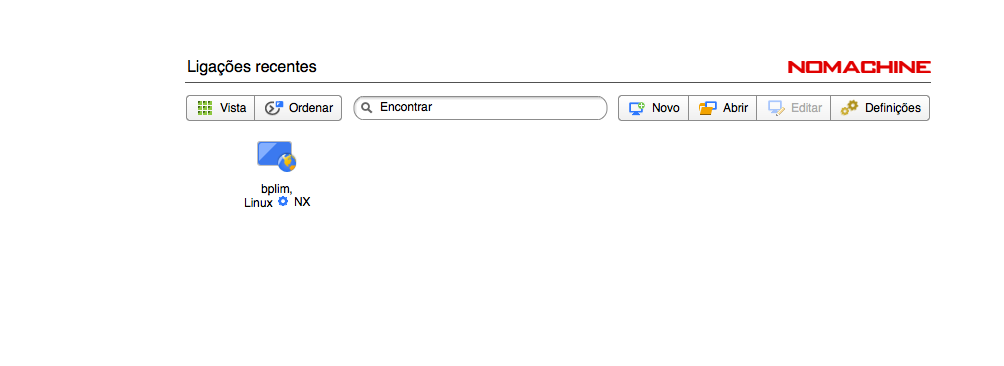
\includegraphics[width=0.65\textwidth,height=\textheight]{./media/image1.png}

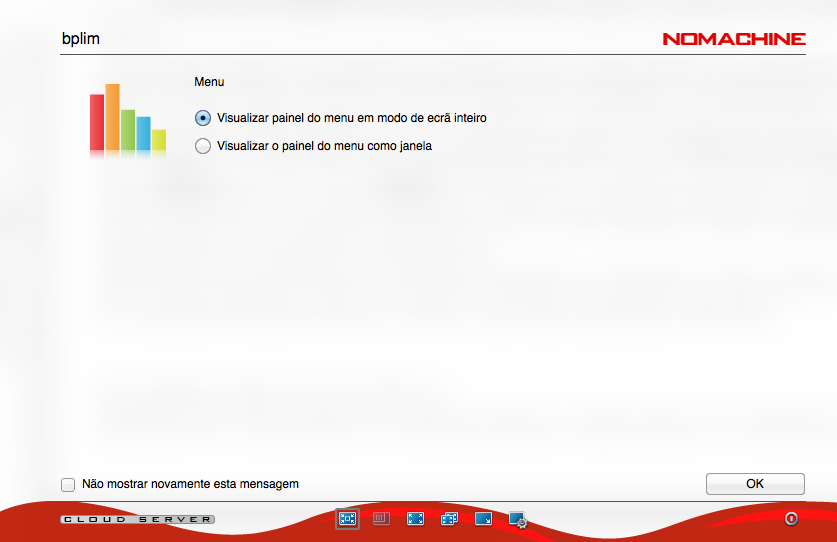
\includegraphics[width=0.65\textwidth,height=\textheight]{./media/image2.png}


\includegraphics[width=0.65\textwidth,height=\textheight]{./media/image3.png}

\begin{enumerate}
\def\labelenumi{\arabic{enumi}.}
\setcounter{enumi}{3}
\tightlist
\item
  Select the ``\textbf{Kickoff Application Launcher}'' menu (in the
  lower left corner):
\end{enumerate}


\includegraphics[width=0.1\textwidth,height=\textheight]{./media/image4.png}

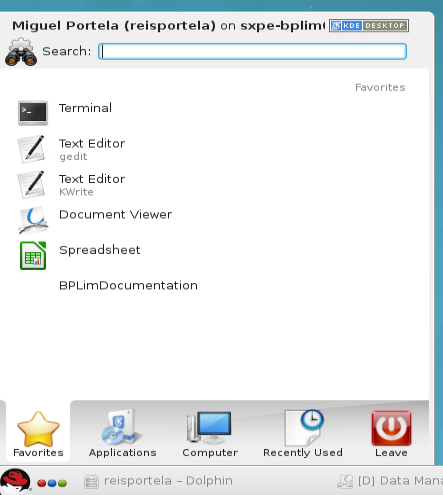
\includegraphics[width=0.5\textwidth,height=\textheight]{./media/image5.png}

\begin{enumerate}
\def\labelenumi{\arabic{enumi}.}
\setcounter{enumi}{4}
\tightlist
\item
  Then you should:
\end{enumerate}

\begin{itemize}
\tightlist
\item
  Click on the ``\textbf{Applications}'' button
\item
  Select \textbf{``BPLIM''} and click on your project (i.e.,
  ``pxxx\_name''). At this stage, you should see a graphical environment
  (`Dolphin' application\footnote{Dolphin is an intuitive and
    easy-to-use file manager. You can use it, for example, to browse the
    directory, to create or delete files/directories (by using the right
    mouse button). For more information about Dolphin, please visit:
    \url{https://userbase.kde.org/Dolphin} .}) like this:
\end{itemize}

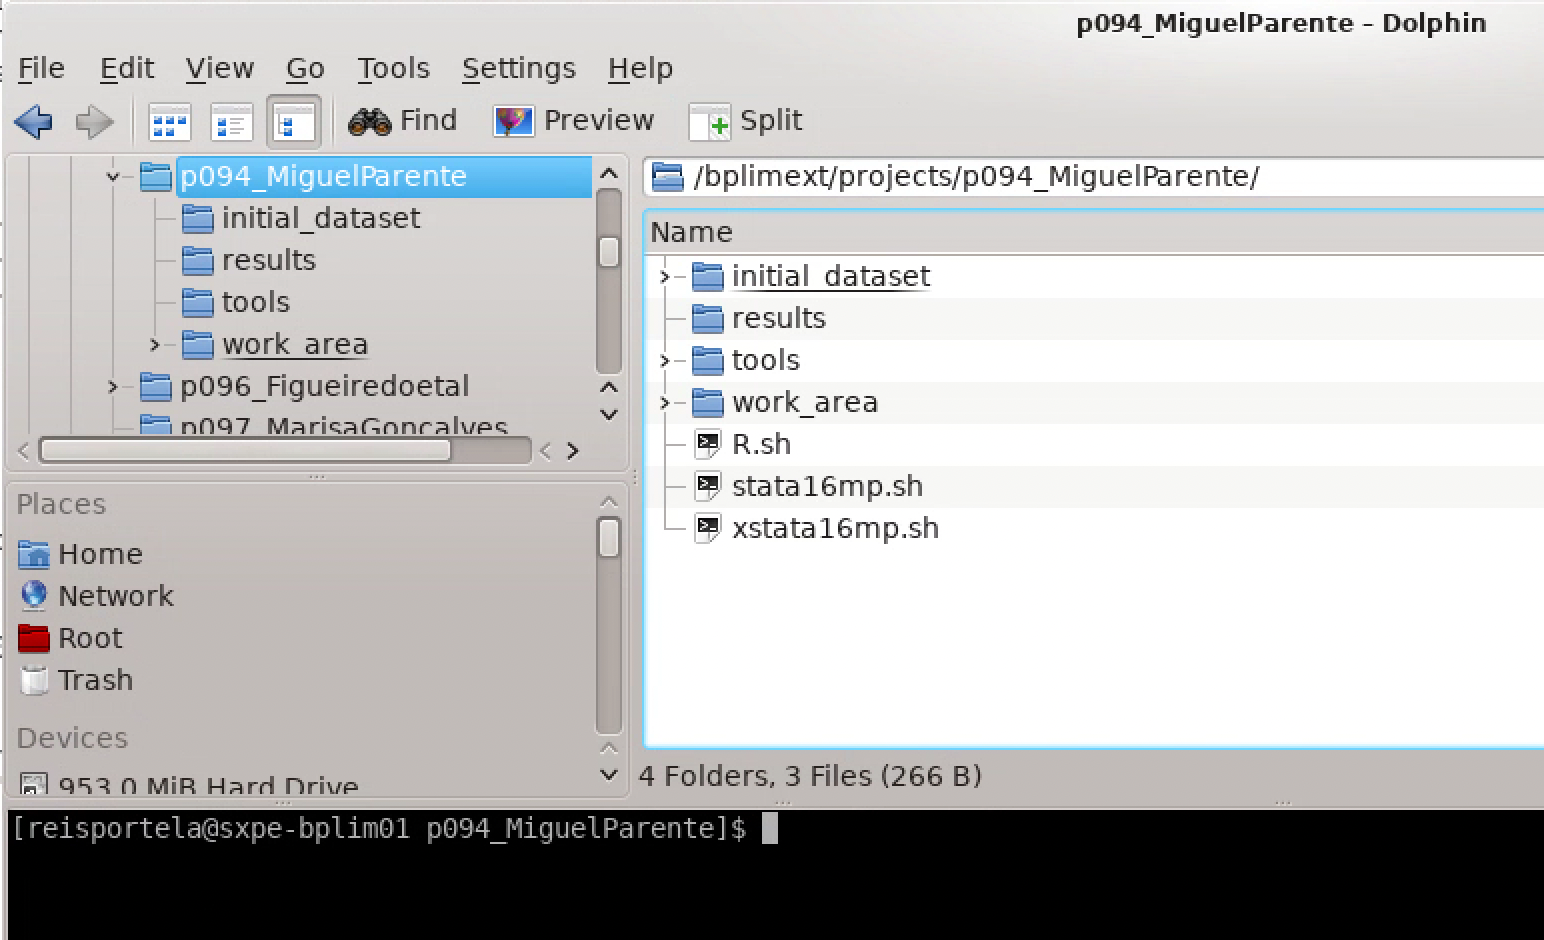
\includegraphics[width=4.72441in,height=2.80866in]{./media/image6.png}

You can see the prompt command line together with `Dolphin' using the
keyboard shortcut `F4'.

\begin{quote}
\begin{enumerate}
\def\labelenumi{\alph{enumi}.}
\setcounter{enumi}{2}
\tightlist
\item
  Files with the "\textbf{sh}" extension allow you to send commands to
  your operating system or to enter your operating system for
  interactive use (for example, the file \emph{xstata17mp.sh} will
  launch the graphical version of Stata 17). You can start the
  application by double-clicking the file name in `Dolphin'\footnote{In
    case `xstata17mp.sh' does not launch Stata please see
    `\protect\hyperlink{statistical_software}{Section 3}'.} or by typing
  in the Terminal \texttt{xstata17mp.sh}
\end{enumerate}
\end{quote}

\begin{enumerate}
\def\labelenumi{\arabic{enumi}.}
\setcounter{enumi}{5}
\tightlist
\item
  The directories that you have access to within the folder include:
\end{enumerate}

\begin{longtable}[]{@{}
  >{\raggedright\arraybackslash}p{(\columnwidth - 2\tabcolsep) * \real{0.5000}}
  >{\raggedright\arraybackslash}p{(\columnwidth - 2\tabcolsep) * \real{0.5000}}@{}}
\toprule\noalign{}
\endhead
\bottomrule\noalign{}
\endlastfoot
\textbf{initial\_dataset} & Data sources provided by BPLIM.

\emph{You have read-only access to this directory.} \\
\textbf{initial\_dataset/modified} & Modified data provided by BPLIM. \\
\textbf{results} & Output files that researchers wish to generate and
extract from the server.

\emph{You have read-write access to this directory.} \\
\textbf{tools} & Specific analysis tools.

\emph{You have read-only access to this directory.} \\
\textbf{work\_area} & Temporary work directory.

\emph{You have read-write access to this directory.} \\
\textbf{/bplimext/doc/Manuals} & Manuals and auxiliary files are
available here. \\
\end{longtable}

\begin{itemize}
\tightlist
\item
  You will have in your \textbf{work\_area} folder templates for both
  Stata and R(\texttt{R.sh}). By default, the template file is
  read-only.
\end{itemize}

\begin{enumerate}
\def\labelenumi{\arabic{enumi}.}
\setcounter{enumi}{6}
\tightlist
\item
  To reset and disconnect the remote desktop connection or session, you
  can simply log out of your remote session, as shown in the screenshot
  below. After you log out, close the window.\footnote{Click on the
    cross button at the upper right corner to close.}
\end{enumerate}

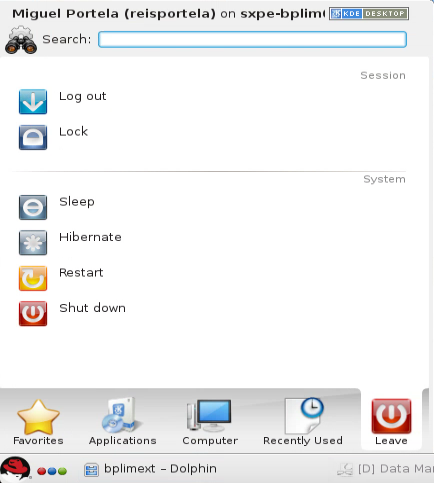
\includegraphics[width=3.14961in,height=3.50521in]{./media/image7.png}

Confirm before exiting by clicking on the \textbf{``Logout''} button to
close the window:\footnote{Note that before exiting the server, you need
  to make sure that all active programs have been closed (unless they
  have been launched in \emph{batch} mode). Running programs in
  \emph{batch} mode is justified for procedures that require high
  computational resources, intense calculation and/or long processing
  time.}

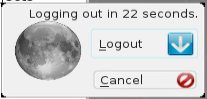
\includegraphics[width=1.14236in,height=0.52288in]{./media/image8.png}

\begin{itemize}
\tightlist
\item
  In case you do not logout, your session will be left open until your
  next login. You may use this facility to run your programs. However,
  one must be aware that this option uses resources from the server, so
  the efficient solution to run your programs ``overnight'' is using the
  batch mode as described in Step 6 below. Furthermore, in case the
  server is rebooted during a maintenance procedure, your session will
  be automatically closed, and unsaved documents will be lost. We
  recommend you save at regular intervals your statistical programs.
\end{itemize}

\pagebreak

\hypertarget{important-guidelines}{%
\section{Important guidelines}\label{important-guidelines}}

\hypertarget{keep-your-home-area-tidy}{%
\subsection{Keep your home area tidy}\label{keep-your-home-area-tidy}}

\begin{itemize}
\item
  \emph{Do not save files in your home area} \texttt{/home/USER\_LOGIN}.
  \emph{In case you exceed its size you will not be able to login.}
\item
  Check regularly the size of your project on the harddrive. Open a
  Terminal and apply the following steps:
\end{itemize}

\begin{enumerate}
\def\labelenumi{\arabic{enumi}.}
\tightlist
\item
  Move to the project folder:
  \texttt{cd\ /bplimext/projects/p000\_xxx\_yyy/}
\item
  List project size: \texttt{du\ -h}
\item
  Check size by folder and list folders with at least 1Gb:
  \texttt{du\ -\/-max-depth\ 1\ -h\ \textbar{}\ sort\ -n\ \textbar{}\ grep\ G}
\item
  Move to the folder `work\_area': \texttt{cd\ work\_area}
\item
  Repeat the check in this folder:
  \texttt{du\ -\/-max-depth\ 1\ -h\ \textbar{}\ sort\ -n\ \textbar{}\ grep\ G}
\item
  Identify duplicated and temporary files and delete them: use the
  command \texttt{rm}
\item
  Compress big files/folders you are not using at the moment:
\end{enumerate}

\begin{quote}
Compress folders: \texttt{tar\ -zcvf\ YOUR\_FOLDER.tar.gz\ YOUR\_FOLDER}

Compress individual files: \texttt{gzip\ YOUR\_FILE}
\end{quote}

\hypertarget{using-the-terminal}{%
\subsection{Using the Terminal}\label{using-the-terminal}}

Linux's Terminal is a command-line interpreter. You can use the `shell'
for a wide range of tasks, including searching files and files'
contents, organizing your working space, and, most importantly, running
your programs in \texttt{batch} mode.

\begin{enumerate}
\def\labelenumi{\arabic{enumi}.}
\tightlist
\item
  Linux's Terminal can be accessed from\footnote{The '\emph{shell'}
    supports the commands in Linux operating system (some are disabled).}
\end{enumerate}

RedHat \textgreater{} Applications \textgreater{} System \textgreater{}
Terminal

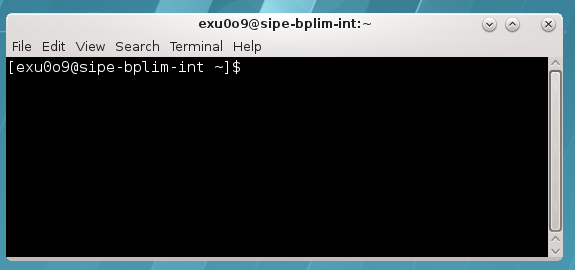
\includegraphics[width=3.93701in,height=1.84868in]{./media/image9.png}

\begin{enumerate}
\def\labelenumi{\arabic{enumi}.}
\setcounter{enumi}{1}
\item
  See \protect\hyperlink{shell_commands}{Section 8.1} for a list of some
  of the most used commands.
\item
  If you use a non-English keyboard, the `true' keyboard might be
  different from the one you see. The changes apply mostly to the
  symbols, not letters or numbers. For example, in case you have a
  Portuguese keyboard on your computer the `+' is now in key `?', or the
  `*' is in SHIFT + ?. This issue is specific to the Operating System of
  your computer
\item
  Remember that Linux is case-sensitive: e.g., ``\texttt{LS}'' and
  ``\texttt{ls}'' are treated as different commands.
\item
  You can use the arrow keys to scroll up and down through the commands
  you have entered.
\item
  You can use the ``Tab'' key to complete the command line
  automatically.
\item
  \emph{e.g.}, type the following line to list elements within a folder
  in a `human-readable' format, \texttt{h}, long list format,
  \texttt{l}, in reverse order, \texttt{r}, sort by modification time,
  \texttt{t}, and almost all files, \texttt{A},

  \texttt{ls\ -lArth}
\end{enumerate}

\hypertarget{statistical_software}{%
\section{Statistical software}\label{statistical_software}}

The installation of additional commands/packages must be requested from
the BPLIM team,
\href{mailto:bplim@bportugal.pt}{\nolinkurl{bplim@bportugal.pt}}.
Researchers are not allowed to install new commands/packages on the
server autonomously.

\hypertarget{stata}{%
\subsection{Stata}\label{stata}}

Stata versions available in the server: 15, 16 and 17 (adjust the
following lines to the Stata version you want to use)

\begin{enumerate}
\def\labelenumi{\arabic{enumi}.}
\tightlist
\item
  Stata can be accessed in interactive graphical or non-graphical
  modes.\footnote{The version of Stata on the server has the same
    features as the Stata on Windows or Mac. By default when the Stata
    starts in this way the "working directory" active becomes your
    folder "work\_area".}
\end{enumerate}

\begin{itemize}
\item
  Interactive non-graphical mode

  Move to the desired folder, e.g.,

  \texttt{cd\ /bplimext/projects/I001\_jdoe/}

  and type

  \texttt{stata17-mp}
\end{itemize}

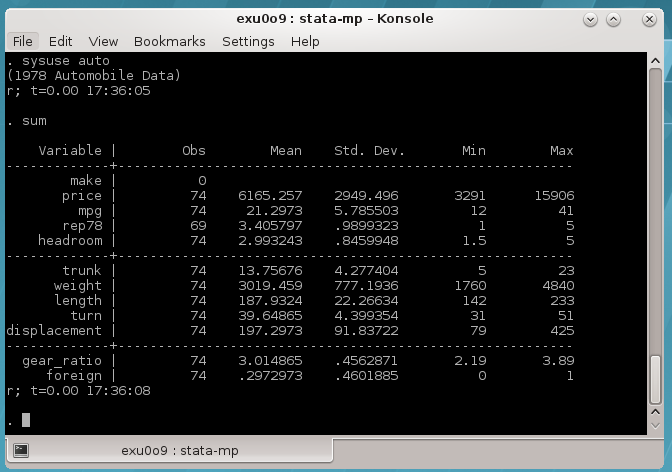
\includegraphics[width=3.54331in,height=2.4886in]{./media/image10.png}

\begin{itemize}
\item
  You may add a `PATH' to your system folder by typing, for example on
  Stata 16, the following command in the shell ``vi
  \textasciitilde/.bash\_profile'' and adapt the following line

  \texttt{PATH=\$PATH:\$HOME/.local/bin:\$HOME/bin:/opt/bplimext/stata17}
\item
  For the interactive graphical mode click on the icons
  ``\textbf{xstata17mp.sh}'' (Stata 17) located in the `desktop',
  depending on the desired Stata version,
\end{itemize}


\includegraphics[width=0.59055in,height=0.46654in]{./media/image11.png}

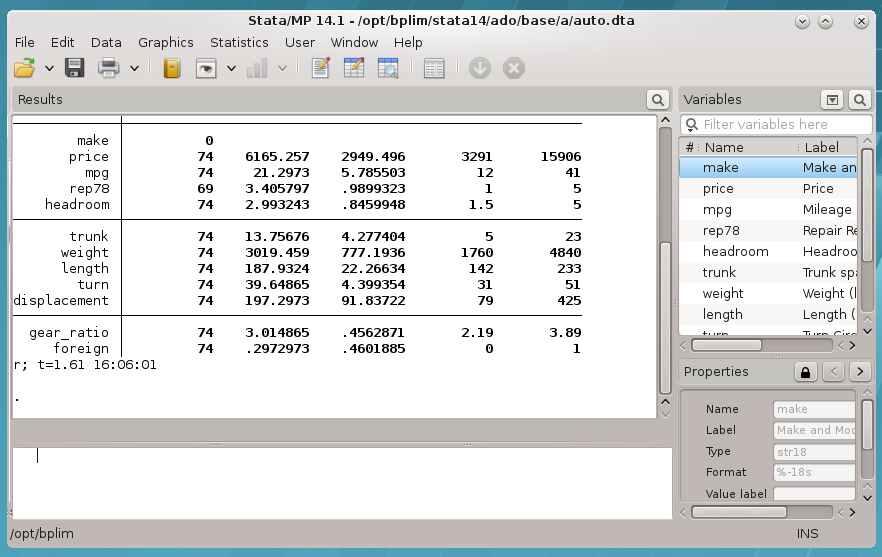
\includegraphics[width=3.93701in,height=2.48638in]{./media/image12.png}

\begin{itemize}
\item
  You can use the `Do-file Editor' in Stata to create your own
  ``do-files'' and ``ado-files'', or you can use \emph{KWrite} editor
  (or `gedit')
\item
  You can open it from \textbf{RedHat} \textgreater{}
  \textbf{Applications} \textgreater{} \textbf{Utilities} \textgreater{}
  \textbf{KWrite}. You can also launch `KWrite' from the `shell' by
  typing `kwrite'
\item
  In case the Stata's icon is not on your desktop, use Dolphin, move to
  the folder `/bplimext/scripts/wrappers/', and drag and drop the file
  `xstata17-mp' into the desktop
\end{itemize}

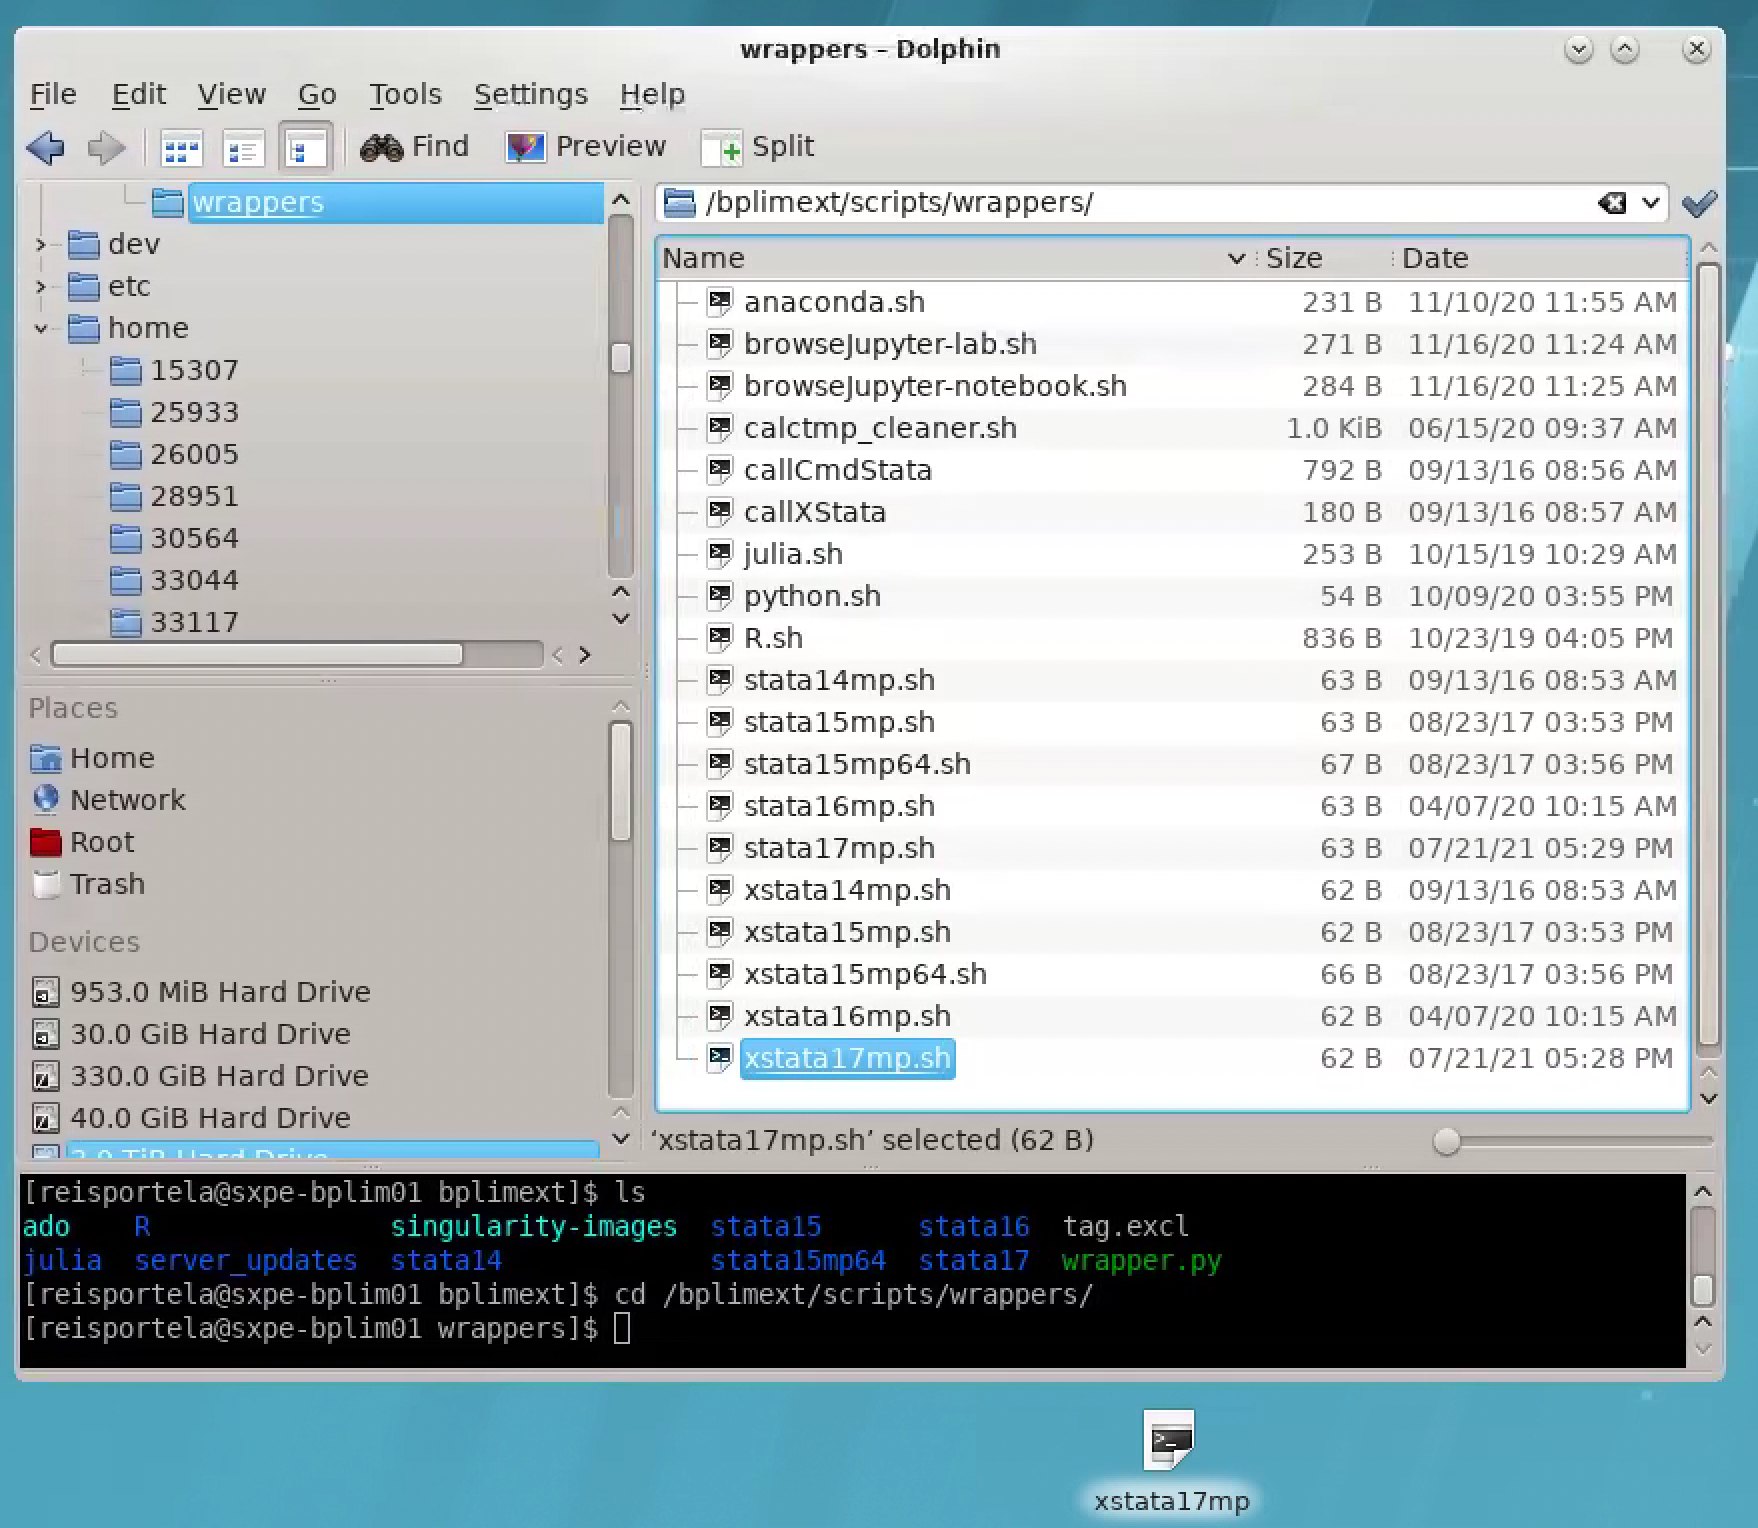
\includegraphics[width=3.93701in,height=2.48638in]{./media/image12b.png}

\textbf{NOTE}: to start Stata use the shortcuts in your project's
folder.

\begin{enumerate}
\def\labelenumi{\arabic{enumi}.}
\setcounter{enumi}{1}
\tightlist
\item
  To look for \textbf{``ado-files''}:
\end{enumerate}

``Ado-files'' are text files containing the Stata program. It is
advisable that one create and save his/her ``ado-files'' so the results
can be replicated later by running the saved ``ado-files'' on the
BPLIM's datasets.

Stata looks for ``ado-files'' in several places. When it comes to
personal ado-directories, they can be categorized in four ways:

\begin{itemize}
\item
  (SITE), the directory for ``ado-files'' your site might have
  installed;
\item
  (PLUS), the directory for ``ado-files'' you might have installed;
\item
  (PERSONAL), the directory for ``ado-files'' you might have written;
\item
  (OLDPLACE), the directory where Stata users used to save their
  personally written ado-files.
\end{itemize}

The ado-files you have just written or those created for this project
can be found in the current directory (.).

Specific `ado-files' you may ask to be made available in the server will
be placed in your folder `/bplimext/projects/YOURPROJECTID/tools'. You
should add this folder to your Stata `ado-files' folder by executing the
following command within Stata,

\texttt{sysdir\ set\ PERSONAL\ "/bplimext/projects/YOURPROJECTID/tools"}

You may also edit your `profile.do' file, located in your root folder,
``/home/YOURPROJECTID/'', and add key instructions you may want to be
executed every time you start Stata. The above instruction is one of
such cases. You can create or edit the file `profile.do' using `Do-file
Editor' within Stata (`vi profile.do' or KWrite are also a possibility).

The \textbf{\emph{sysdir}} command within Stata will tell you where they
are on your computer:

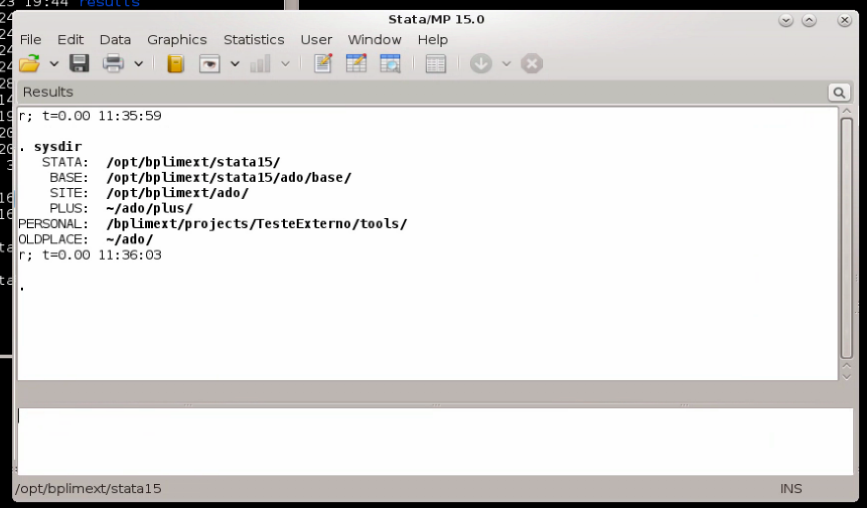
\includegraphics[width=3.93681in,height=2.27514in]{./media/image13.png}

\begin{enumerate}
\def\labelenumi{\arabic{enumi}.}
\tightlist
\item
  Start a \emph{\textquotesingle{}\textbf{shell}\textquotesingle{}} in
  Linux and navigate to the directory of the ``do-file'' file that you
  want to run (ex: prog1.do)
\end{enumerate}

\texttt{cd\ /bplimext/projects/I001\_jdoe/work\_area/}

\begin{enumerate}
\def\labelenumi{\arabic{enumi}.}
\setcounter{enumi}{1}
\tightlist
\item
  You might find it easier to use `Dolphin' (= File Manager) to move
  over your folder structure. In this case, we recommend activating the
  `shell' (= `Terminal') associated with `Dolphin'
\end{enumerate}

\begin{itemize}
\item
  use Dolphin/File Manager
\item
  click `F4' to activate the shell with Dolphin. Benefit: fast
  transition within folders and, at the same time, the ability to run
  shell commands
\end{itemize}

\begin{enumerate}
\def\labelenumi{\arabic{enumi}.}
\setcounter{enumi}{2}
\item
  Create an ASCII file named, e.g., `batch\_prog1'
\item
  Inside the file, write just a line with the execution command you
  would type in the `shell'; e.g.,

  \texttt{/bplimext/projects/I001\_jdoe/stata-mp\ do}

  \texttt{/bplimext/projects/I001\_jdoe/work\_area/prog1.do}
\item
  You can use, for example, the command line app `vi' to create the
  batch file
\end{enumerate}

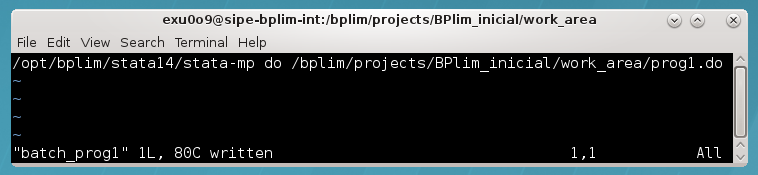
\includegraphics[width=3.54331in,height=0.81802in]{./media/image14.png}

\begin{enumerate}
\def\labelenumi{\arabic{enumi}.}
\setcounter{enumi}{5}
\tightlist
\item
  The batch file can also be created using apps like `kwrite' or Stata
  `do file editor'
\end{enumerate}

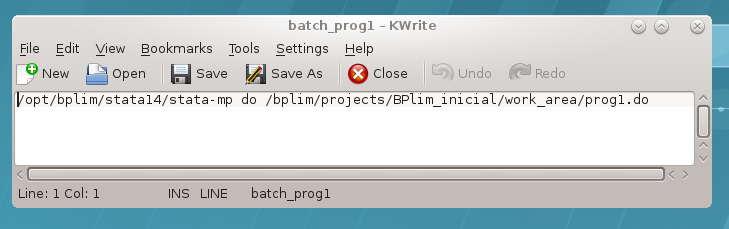
\includegraphics[width=3.54331in,height=1.11324in]{./media/image15.png}

or

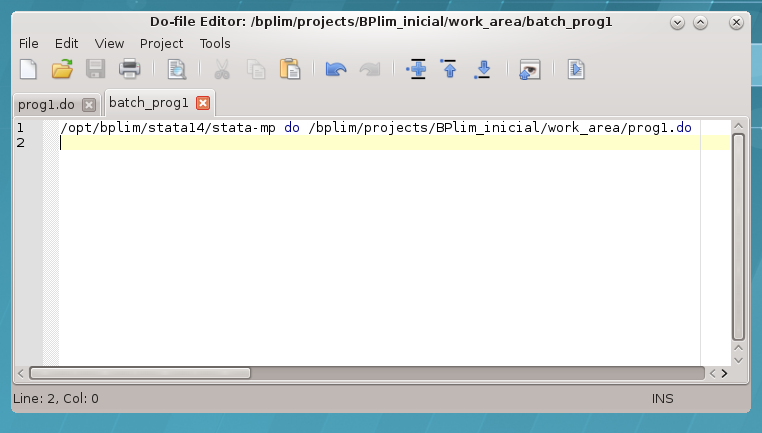
\includegraphics[width=3.54331in,height=2.01342in]{./media/image16.png}

\begin{enumerate}
\def\labelenumi{\arabic{enumi}.}
\setcounter{enumi}{6}
\item
  You may add the extension `.txt' to the name of the batch file, as
  sometimes Stata \emph{doeditor} does not `see' the file `batch', while
  it `sees' `batch.txt'
\item
  Once the batch file is created, one runs the \texttt{.do} file in
  batch mode by typing in the `Terminal':

  \texttt{at\ now\ -f\ batch.txt}
\item
  Type `man at' to see a further option of the command `\texttt{at}';
  e.g., one could type

  \texttt{at\ now\ +\ 5\ hours\ -f\ batch.txt}
\end{enumerate}

or

\begin{verbatim}
`at now + 4 minutes -f batch_prog1`
\end{verbatim}

to run the Stata program within 5 hours or 4 minutes from now,
respectively. `\texttt{man}' is the help function in Linux

\begin{enumerate}
\def\labelenumi{\arabic{enumi}.}
\setcounter{enumi}{9}
\item
  Type `\texttt{top}' in the shell/Terminal to confirm the program is
  running
\item
  Under `\texttt{top}' type `\texttt{i}' to hide irrelevant processes
  (show less output)
\item
  To kill a running process with `\texttt{top}' press `\texttt{k}', for
  `\texttt{kill}', write \textgreater{} the process number and then type
  `\texttt{9}'. The process number is \textgreater{} identified in the
  first column as PID
\item
  To get out of the \texttt{top}, type `\texttt{q}'
\item
  Useful features of the command `\texttt{at}':
\end{enumerate}

\begin{itemize}
\item
  `\texttt{atq}': use it to see programs in the batch queue (an
  `\texttt{=}' sign indicates the program is running; an `\texttt{a}'
  indicates it is in the queue and we see the time when it will be
  executed)
\item
  `\texttt{atrm} \#': remove a batch from the batch queue
\item
  one can see how the batch is running by typing

  \texttt{tail\ -\/-f\ logcrc\_may21.log}
\end{itemize}

It allows you to see an updated version of the last lines of the log;
\emph{i.e.}, it updates each time Stata changes the log. A key advantage
of \texttt{tail} is that it does not interfere with the log file.
Namely, it does not write over it.

\begin{enumerate}
\def\labelenumi{\arabic{enumi}.}
\setcounter{enumi}{14}
\tightlist
\item
  Another way to run a program in the background is by using the command
  `\texttt{screen}'
\end{enumerate}

\begin{itemize}
\item
  `\texttt{screen}' is useful when one wants to run Stata in interactive
  mode and still guarantees that if the network connection goes down one
  does not lose the session. We can simply kill the `NoMachine' session
  and recover it later by typing `\texttt{screen\ -\/-r}'
\item
  We can run several instances of \texttt{screen}. If this is the case,
  after opening a new NoMachine session, we need to type in the Terminal
  shell `\texttt{screen\ -d}' to identify the running background
  sessions. We can retrieve a particular session by knowing the
  `\texttt{pid}' number and typing `\texttt{screen\ -r\ 34176}'
\end{itemize}

\hypertarget{r}{%
\subsection{R}\label{r}}

\begin{enumerate}
\def\labelenumi{\arabic{enumi}.}
\tightlist
\item
  As with Stata, R can be accessed in interactive graphical or
  non-graphical modes.
\end{enumerate}

\begin{itemize}
\tightlist
\item
  Interactive non-graphical mode: go to the RedHat symbol and type `R'
  in the Search box
\end{itemize}

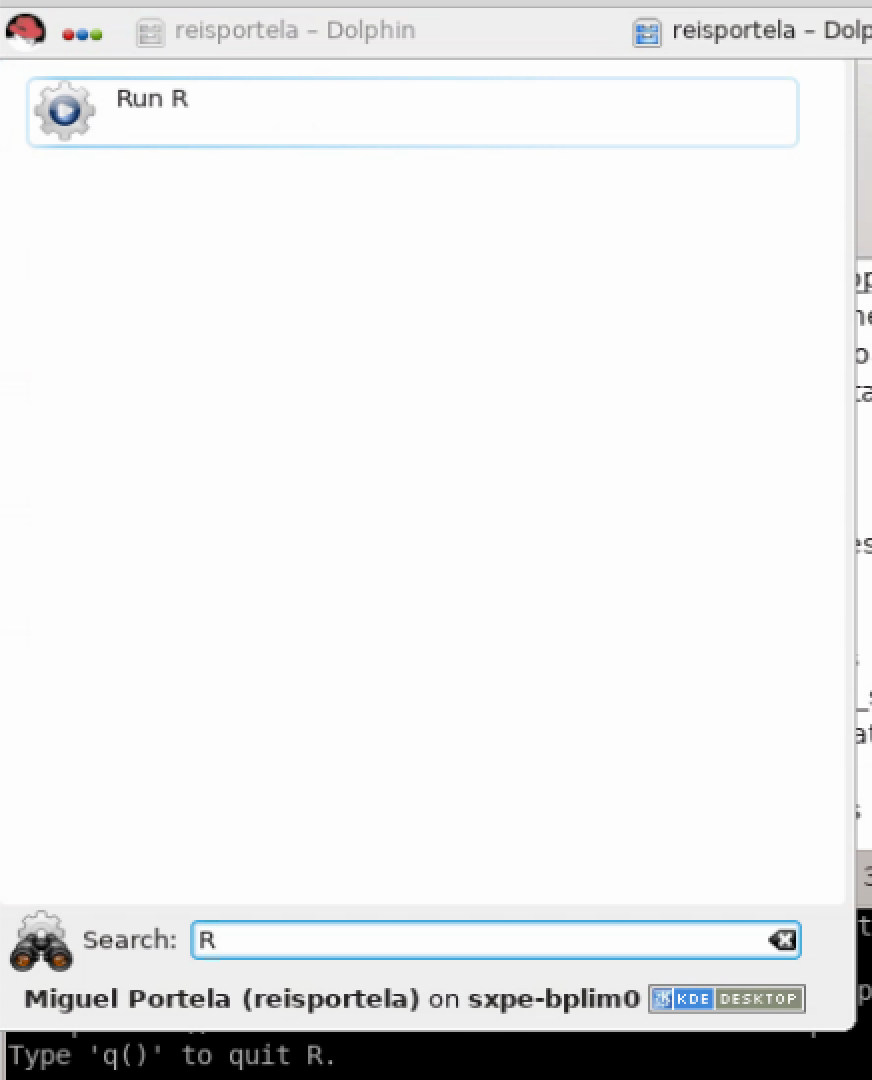
\includegraphics[width=0.5\textwidth,height=\textheight]{./media/CallR.png}

\begin{itemize}
\tightlist
\item
  Alternatively, you can open a Terminal and type
\end{itemize}

\begin{quote}
\texttt{R}
\end{quote}

\begin{itemize}
\tightlist
\item
  Please make sure R is in your PATH; type \texttt{\$PATH} in the
  Terminal. If this is not the case, type \texttt{PATH=\$PATH:/usr/bin/}
\end{itemize}

\begin{enumerate}
\def\labelenumi{\arabic{enumi}.}
\setcounter{enumi}{1}
\tightlist
\item
  Using RStudio.
\end{enumerate}

\begin{itemize}
\tightlist
\item
  Open a Terminal and type
\end{itemize}

\begin{quote}
\texttt{rstudio}
\end{quote}

\begin{itemize}
\tightlist
\item
  Please make sure RStudio is in your PATH; type \$PATH in the Terminal.
  If this is not the case, type
\end{itemize}

\begin{quote}
\texttt{PATH=\$PATH:/opt/bplimext/R/usr/lib64/rstudio/bin/}
\end{quote}

\begin{itemize}
\tightlist
\item
  In case you face difficulties opening/saving files in RStudio, please
  open a Terminal and type
\end{itemize}

\begin{quote}
\texttt{/bplimext/scripts/wrappers/R.sh}
\end{quote}

\textbf{IMPORTANT}: do not save your workspace image in your home folder
(\texttt{Save\ workspace\ image?\ {[}y/n/c{]}}). If you want to keep the
workspace file save it in your project folder under \texttt{work\_area}.

\textbf{RStudio Font Type}: please make sure you are not using Font Type
Courier (Menu Tools, Global Options, Appearance \ldots)

\hypertarget{python}{%
\subsection{Python}\label{python}}

\begin{enumerate}
\def\labelenumi{\arabic{enumi}.}
\tightlist
\item
  Open a Terminal and type
\end{enumerate}

\begin{quote}
\texttt{python3}
\end{quote}

\hypertarget{julia}{%
\subsection{Julia}\label{julia}}

\hypertarget{alternative-a}{%
\subsubsection{Alternative A}\label{alternative-a}}

\begin{enumerate}
\def\labelenumi{\arabic{enumi}.}
\tightlist
\item
  Open a Terminal and type (\texttt{julia} is located in
  /opt/bplimext/julia/lib/, you can add it to your \texttt{PATH})
\end{enumerate}

\begin{quote}
\texttt{julia}
\end{quote}

\begin{enumerate}
\def\labelenumi{\arabic{enumi}.}
\setcounter{enumi}{1}
\tightlist
\item
  Use Atom: open a Terminal and type
\end{enumerate}

\begin{quote}
\texttt{atom}
\end{quote}

\hypertarget{alternative-b-using-a-container-see-the-discussion-in-the-appendix}{%
\subsubsection{Alternative B: using a container (see the discussion in
the
Appendix)}\label{alternative-b-using-a-container-see-the-discussion-in-the-appendix}}

\begin{enumerate}
\def\labelenumi{\arabic{enumi}.}
\tightlist
\item
  Request a container with \textbf{\texttt{Julia}} for your project
\end{enumerate}

\begin{quote}
The container will be in the folder \texttt{tools} inside the project
folder
\end{quote}

\begin{quote}
\textbf{Advantages}: you can build a Julia setup fine-tuned to your
project, including the definition of Julia's version and packages
\end{quote}

\hypertarget{updates-to-the-commands-and-packages-list}{%
\subsection{Updates to the commands and packages
list}\label{updates-to-the-commands-and-packages-list}}

Additional commands/packages or updates to the existing ones have to be
requested from BPLIM's Team.

\hypertarget{build-a-container-to-fine-tune-your-statistical-packages}{%
\subsection{Build a container to fine-tune your statistical
packages}\label{build-a-container-to-fine-tune-your-statistical-packages}}

You can use Singularity containers in the server. To do so, please send
us the definition file so we build the image and put it in your working
area. You can find detailed information on Singularity containers at
\url{https://sylabs.io/}. We provide some notes in the Appendix

\hypertarget{allowed-outputs}{%
\section{Allowed outputs}\label{allowed-outputs}}

Stata results can be exported to a file on disk using one of the
following formats:

\begin{enumerate}
\def\labelenumi{\arabic{enumi}.}
\item
  ASCII files: e.g., log files
\item
  graphs: as \texttt{.PNG} (do not use the option save, or saving,
  within a graph command; instead, use the separate command line `graph
  export xyz.png')
\item
  csv: CSV (Comma Separated Value format), \emph{e.g.}, for use with MS
  Excel
\item
  rtf: Rich Text Format for use with word processors
\item
  xls or xlsx: Excel files with output tables
\item
  tex: \LaTeX format
\end{enumerate}

\hypertarget{removing-outputs}{%
\section{Removing outputs}\label{removing-outputs}}

The output files, e.g., log files or images, must be requested from the
BPLIM team,
\href{mailto:bplim@bportugal.pt}{\nolinkurl{bplim@bportugal.pt}}.
Researchers are not allowed to place or remove files on the server
autonomously.

Place in the ``\ul{results}'' folder all the outputs you want to remove
from the server.\footnote{You may only remove text files that do not
  contain data or results that allow identification. For all the graphs
  you request as an output you must provide the corresponding Table to
  replicate it. You may only export graphs in .PNG format (no vector
  graph is allowed).}

\begin{enumerate}
\def\labelenumi{\arabic{enumi}.}
\item
  Send an email with the title ``\textbf{project I001\_jdoe}: request
  for result extraction'' to ``\textbf{\ul{bplim@bportugal.pt}}''.
\item
  Upon validation, the results will be sent to you via email.
\end{enumerate}

\hypertarget{users-home-folder}{%
\section{User's Home folder}\label{users-home-folder}}

\begin{enumerate}
\def\labelenumi{\arabic{enumi}.}
\item
  Do not save files in your Home folder: ``/home/USER\_ID/''.
\item
  Regularly clean your Trash folder. If your disk use goes over the
  quota, you will be prevented from login in. In the Terminal type:

  \texttt{rm\ -rf\ \textasciitilde{}/.local/share/Trash/*}
\end{enumerate}

\hypertarget{scientific-support}{%
\section{Scientific support}\label{scientific-support}}

Researchers will be provided with the necessary scientific and
computational support (\emph{i.e.}, advises on programming,
computational resources, micro econometrics, and econometrics of panel
data for research undertaken with the selected microdata).

\hypertarget{appendix}{%
\section{Appendix}\label{appendix}}

\hypertarget{shell_commands}{%
\subsection{Basic `shell' commands on Linux}\label{shell_commands}}

\begin{itemize}
\item
  \texttt{top}: List the procedures that are being executed on the
  server

  \begin{itemize}
  \item
    press `\texttt{i}' option to omit background processes;
  \item
    clicar press `\texttt{h}' para \textbf{\emph{help on top options}} ;
    `\texttt{h}' \textgreater{} option to obtain the \textbf{top command
    help}.
  \end{itemize}
\item
  \texttt{pwd}: Show current working directory
\item
  \texttt{cd}: Change directory

  \texttt{cd\ /bplimext/projects/I001\_jdoe/work\_area/}

  `\texttt{cd\ \textasciitilde{}}' moves to your home folder
\end{itemize}

\begin{itemize}
\item
  \texttt{cp}: Copy file(s) to a given path

  \texttt{cp\ prog1.do\ /bplimext/projects/I001\_jdoe/results}
\end{itemize}

\begin{itemize}
\item
  \texttt{mv}: Move file(s) or rename a file from a given path

  \texttt{mv\ prog1.do\ /bplimext/projects/I001\_jdoe/results}
\end{itemize}

\begin{itemize}
\item
  \texttt{rm}: Delete a file

  \texttt{rm\ /bplimext/projects/I001\_jdoe/results/prog1.do}
\end{itemize}

\begin{itemize}
\item
  \texttt{mkdir}: Creates a directory

  \texttt{mkdir\ programs}
\end{itemize}

\begin{itemize}
\item
  \texttt{rmdir}: Deletes a directory

  \texttt{rmdir\ programs}
\end{itemize}

\begin{itemize}
\item
  \texttt{screen}: Switch between screen

  \texttt{screen\ top}
\end{itemize}

\begin{itemize}
\item
  \texttt{man}: Show the manual page for the given command

  \texttt{man\ ls}
\end{itemize}

\begin{itemize}
\tightlist
\item
  \texttt{du\ -h}: Check the information on disk usage of files and
  directories.
\end{itemize}

\begin{quote}
The ``\texttt{-h}'' option with ``\texttt{du}'' command provides results
in ``Human Readable Format''.
\end{quote}

Ex: \texttt{du\ /bplimext/projects/I001\_jdoe/work\_area/}

\begin{itemize}
\item
  \texttt{df\ -h}: Check disk space utilization and show the disk space
  \textgreater{} statistics in ``human readable'' format.
\item
  \texttt{vi}: View `ASCII' files; e.g., log files
\item
  \texttt{ghostscript}: Preview files with the extensions of \emph{.eps}
  and \emph{.pdf}
\end{itemize}

\begin{quote}
\texttt{ghostscript\ /bplimext/projects/I001\_jdoe/results/file\_name.pdf}
\end{quote}

\begin{itemize}
\item
  \texttt{okular}: View `PDF'
\item
  \texttt{find}: Find files
\end{itemize}

\begin{quote}
Structure: find /path option filename

\texttt{find\ .\ -name\ "*.do"}

Send the `\texttt{find}' output to a file:

\texttt{find\ .\ -name\ "\textbackslash{}*.do"\ \textgreater{}\ find\_results.txt}

Look for a particular string within the `find' output:

\texttt{find\ .\ -name\ "\textbackslash{}*.do"\ \textbar{}\ grep\ "analysis"}

Identify files with extension `.do' that \textbf{contain} the word
`graph':

\texttt{find\ .\ -name\ "\textbackslash{}*.do"\ -exec\ grep\ "graph\ export"\ \textquotesingle{}\{\}\textquotesingle{}\ \textbackslash{};\ -print}
\end{quote}

\begin{itemize}
\item
  \texttt{passwd}: Change your password
\item
  \textbf{To exit} a program, type \textbf{CTRL + C} (`CTRL + C' kills a
  particular execution in the shell)
\end{itemize}

\hypertarget{using-the-vi-file-editor}{%
\subsection{Using the `vi' file editor}\label{using-the-vi-file-editor}}

\begin{enumerate}
\def\labelenumi{\arabic{enumi}.}
\item
  In the shell type `\texttt{vi\ batch1.txt}'
\item
  These are the main shortcut keys

  \begin{enumerate}
  \def\labelenumii{\alph{enumii}.}
  \item
    `i' insert text
  \item
    `ESC' key get out of the `insert' mode
  \item
    `x' delete specific characters
  \item
    `dd' delete a full line
  \item
    `10 dd' delete 10 lines
  \item
    `yy' copy lines
  \item
    `p' paste lines
  \item
    `SHIFT + G' go to the last line
  \item
    `gg' goes to the first line
  \item
    `ESC + q!' exit `vi' without writing
  \item
    `w!' write and replace the file
  \item
    `ESC + q' exit the `vi' session
  \item
    Check, for example,
    \url{https://www.cs.colostate.edu/helpdocs/vi.html}
  \end{enumerate}
\item
  Much easier solution: call `\texttt{gedit}' file editor
\item
  Linux commands I have to add to the manual
\item
  `CTRL + R': allows me to recover a previous command
\item
  \texttt{vi\ .bash\_history}
\end{enumerate}

\hypertarget{password}{%
\subsection{External server's password requirements}\label{password}}

\begin{longtable}[]{@{}
  >{\raggedright\arraybackslash}p{(\columnwidth - 4\tabcolsep) * \real{0.3288}}
  >{\raggedright\arraybackslash}p{(\columnwidth - 4\tabcolsep) * \real{0.3288}}
  >{\raggedright\arraybackslash}p{(\columnwidth - 4\tabcolsep) * \real{0.3288}}@{}}
\toprule\noalign{}
\endhead
\bottomrule\noalign{}
\endlastfoot
\textbf{Rule} & \textbf{Value} & \textbf{Notes } \\
Maximum Password Lifetime & \textbf{\ul{60 days}} & \emph{After 60 days
the password will expire} and has to be changed in the next login. The
password can be changed at any moment using: \textbf{(1)}, ``All
Applications \textbar{} Settings \textbar{} System Settings -- Account
Details'', click ``Change Password''; or, \textbf{(2)}, in the `Shell'
type `passwd' \\
Minimum Number of Character Classes & 4 &
\begin{minipage}[t]{\linewidth}\raggedright
You should include at least 4 classes of characters in the password. For
example, small letters, capital letters, numbers and punctuation marks.

There are a total of five classes:

\begin{quote}
1. Capital letters : A-Z

2. Small letters: a-z

3. Numbers: 1-9
\end{quote}
\end{minipage} \\
& & \begin{minipage}[t]{\linewidth}\raggedright
\begin{quote}
4. Punctuation marks: \textless space\textgreater{} ! \% \& ( ) * + . ,
\{ \} \[ \] \textasciitilde{} " \# \$ \textquotesingle{} - /
\textbackslash{} \^{} \_ ` \textbar{}

5. Characters above 127 (0x7F): marked characters (ã, á, ä, à, etc.);
symbols (@, £, §, º, ª, «, », etc.)
\end{quote}

Number of characters: by using the same character 3 or more times may
imply the use of an additional class (it is highly recommended that you
do not use consecutively the same character more than 2 times)
\end{minipage} \\
Minimum Length of Password & 8 & The minimum size of the password is 8
characters (it may be higher in case you repeat characters) \\
Password History & 7 & One cannot use a password defined in the previous
set of 7 passwords \\
Maximum Consecutive Failures & 6 & If the user fails 6 consecutive times
the password the account will be locked for the time defined in
``Lockout Time'' \\
Fail Interval & 60 sec. & Time interval for attempts to enter a password
to be considered consecutive. If more than 60 seconds have elapsed since
the last attempt, consecutive attempts are no longer considered, ie the
number of failures, according to the requirement "Maximum Consecutive
Failures" becomes one. \\
Lockout Time & 600 sec. & Time (10 minutes) during which the account
will be locked if the maximum number of failed attempts is reached. \\
\end{longtable}

\hypertarget{install_nomachine}{%
\subsection{Download, install and configure NoMachine
client}\label{install_nomachine}}

\textbf{Step 1}: go to the link below and use the credentials provided
by BPLIM to access the site. \textbf{Note}: sometimes the internet
provider, \emph{e.g.}, a University, may block access to this particular
website. Please check with your provider in case you get an error while
trying to use the link.

\url{https://www.bportugal.pt/webdrive/index.php/s/irAzxZmir8KHyzD/authenticate}

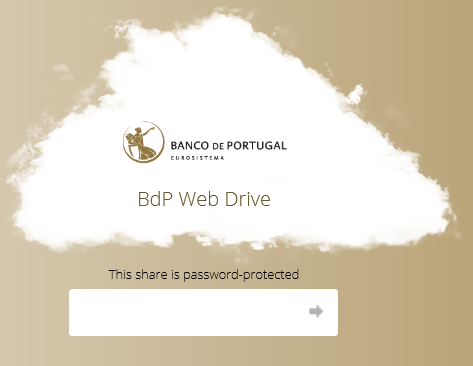
\includegraphics[width=3.0528in,height=2.3622in]{./media/image17.png}

\textbf{Step 2}: download the file with an extension compatible with
your OS (Operation System)

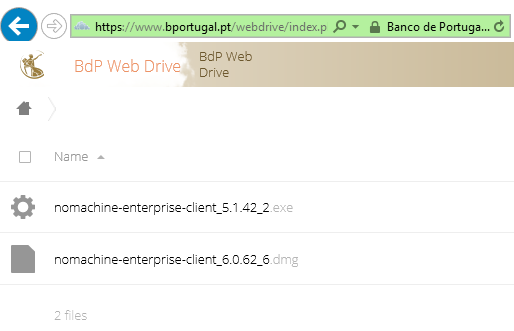
\includegraphics[width=3.6682in,height=2.3622in]{./media/image18.png}

\textbf{Step 3}: install `NoMachine'

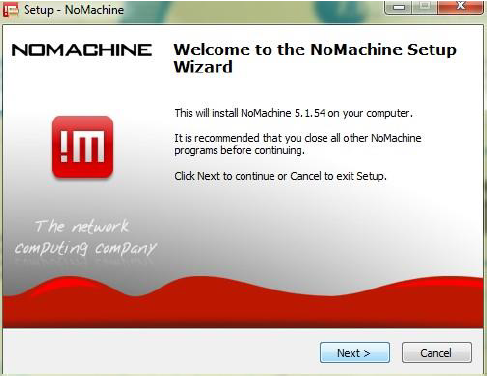
\includegraphics[width=4.07941in,height=3.14961in]{./media/image19.png}

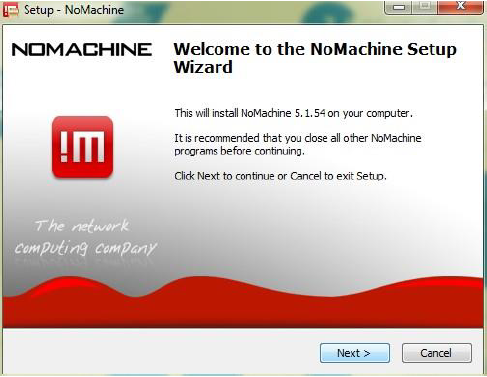
\includegraphics[width=4.06859in,height=3.14961in]{./media/image20.png}

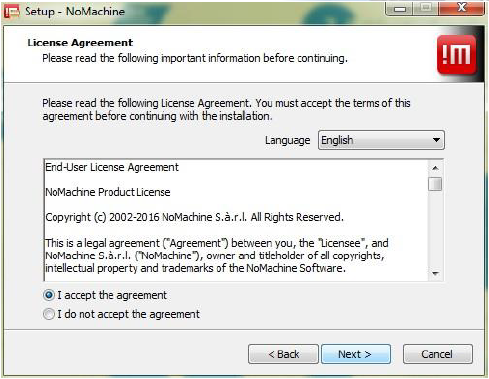
\includegraphics[width=4.06374in,height=3.14961in]{./media/image21.png}

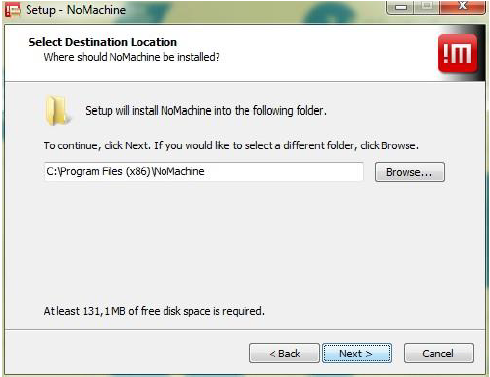
\includegraphics[width=4.09365in,height=3.14961in]{./media/image22.png}

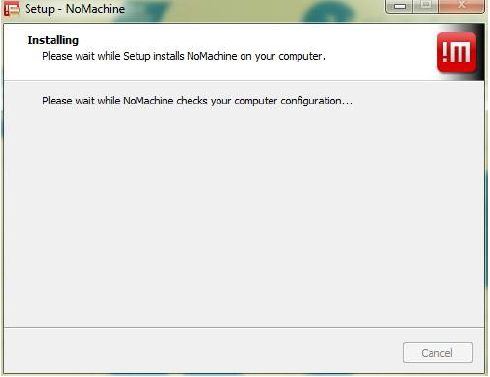
\includegraphics[width=4.09365in,height=3.14961in]{./media/image23.png}

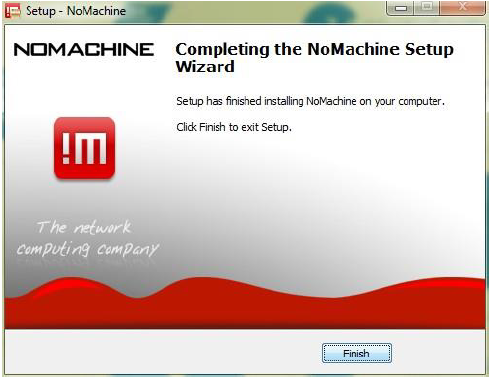
\includegraphics[width=4.09115in,height=3.14961in]{./media/image24.png}

\textbf{\hfill\break
}

\textbf{Step 4}: reboot your computer

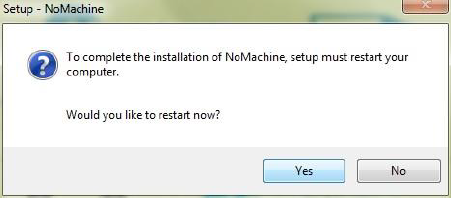
\includegraphics[width=2.75591in,height=1.21602in]{./media/image25.png}

\textbf{Step 5}: NoMachine client access configuration

\textbf{Step 5.1}: start `NoMachine' and create a new connection

\begin{quote}
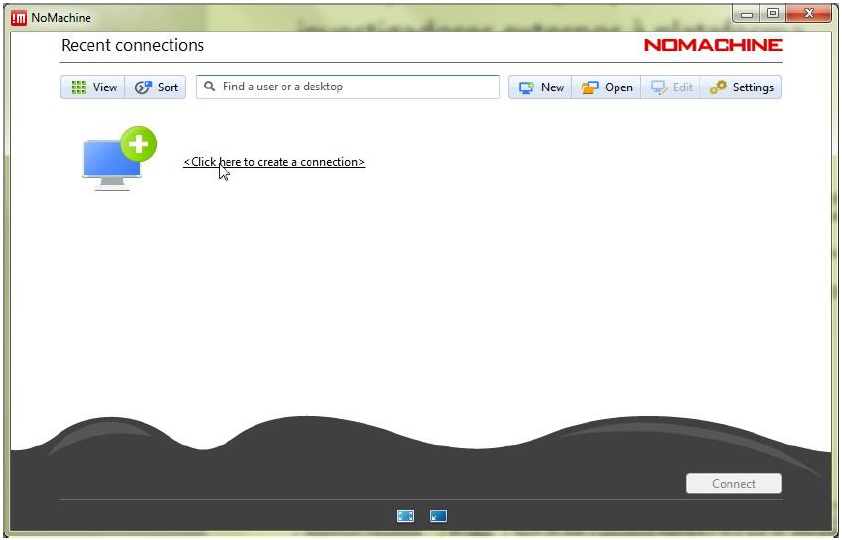
\includegraphics[width=4.72441in,height=3.02971in]{./media/image26.png}
\end{quote}

\textbf{Step 5.2}: Choose `NX protocol'

\begin{quote}
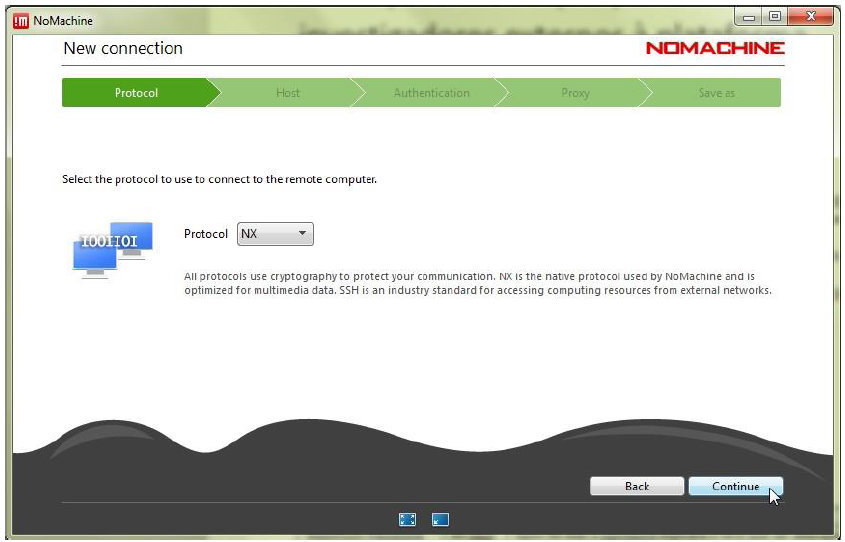
\includegraphics[width=4.72441in,height=3.0302in]{./media/image27.png}
\end{quote}

\textbf{Step 5.3}: Define the `Host' as bplimexterno.bportugal.pt,
`Port' 4000

\begin{quote}
Click `Use UDP communication for multimedia data'

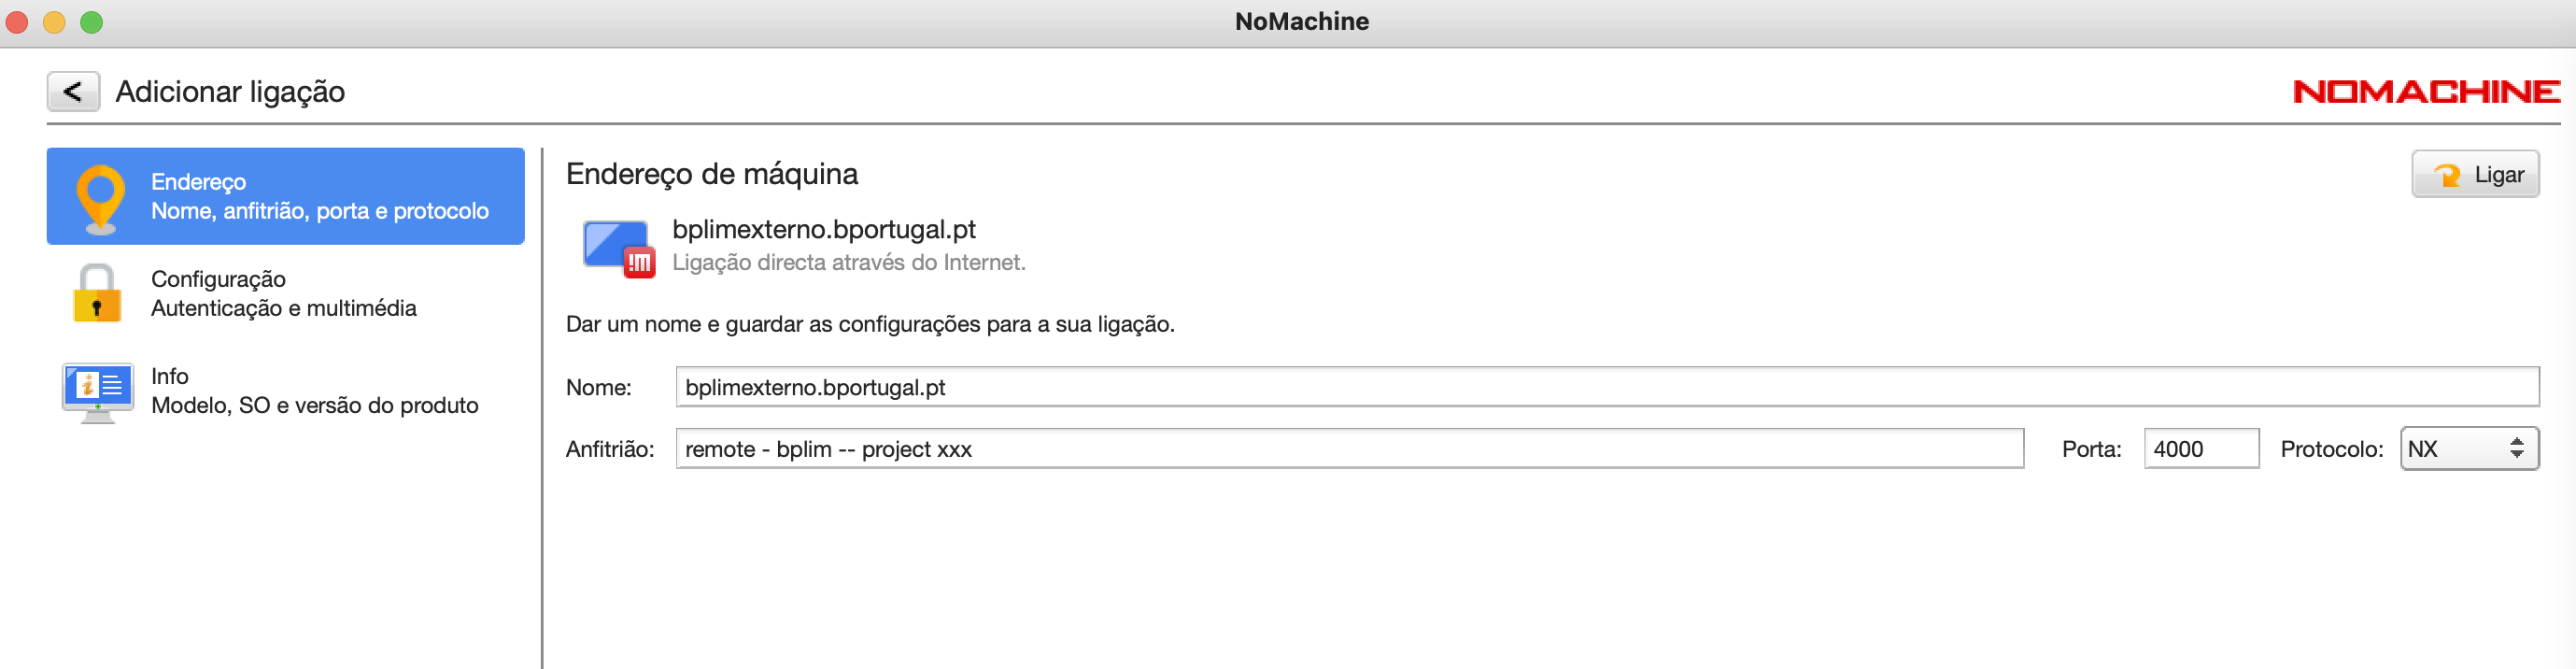
\includegraphics[width=4.72441in,height=3.02002in]{./media/image28_new.png}

\textbf{Step 5.4}: Use password authentication, with or without proxy,
depending on the instructions of the network administrator/user
\textquotesingle s computer support, with the name
``BPLIM-LabInvestMicrodados Banco de Portugal''.

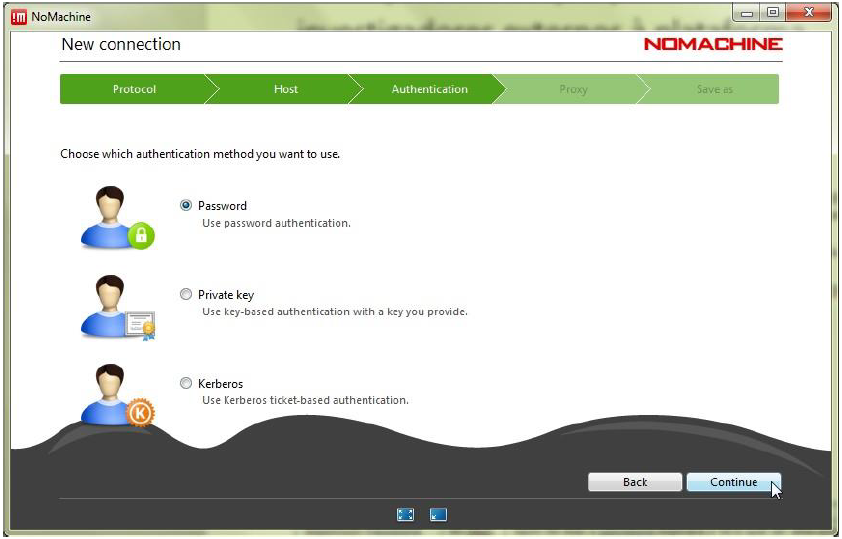
\includegraphics[width=4.72441in,height=3.02438in]{./media/image29.png}

\textbf{Step 5.5}: Do not use a `proxy'

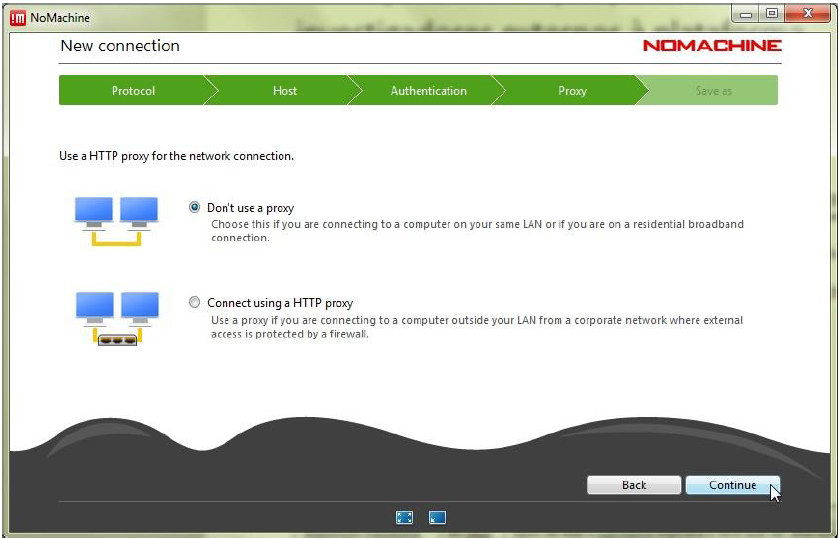
\includegraphics[width=4.72441in,height=3.03165in]{./media/image30.png}

\textbf{Step 5.6}: Define a name for the connection

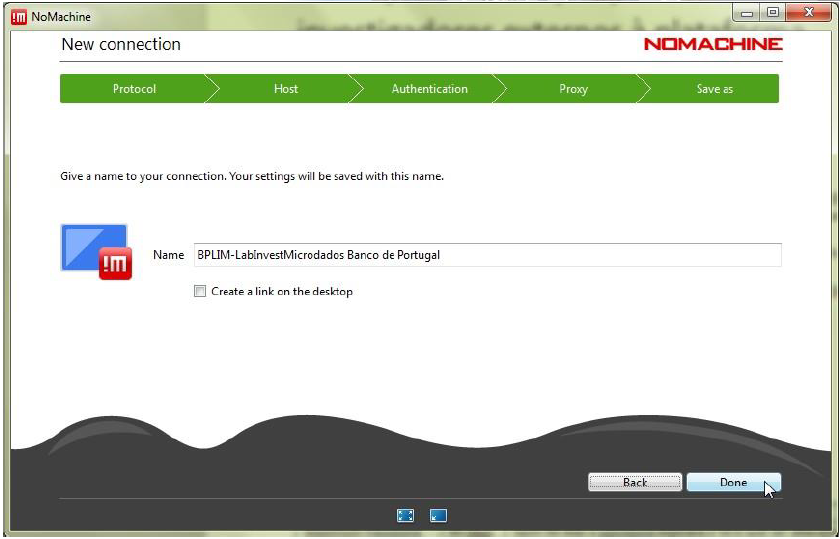
\includegraphics[width=4.72441in,height=3.03165in]{./media/image31.png}

\textbf{Step 5.7}: Once the entry for bplimexterno.bportugal.pt has been
created, connect:

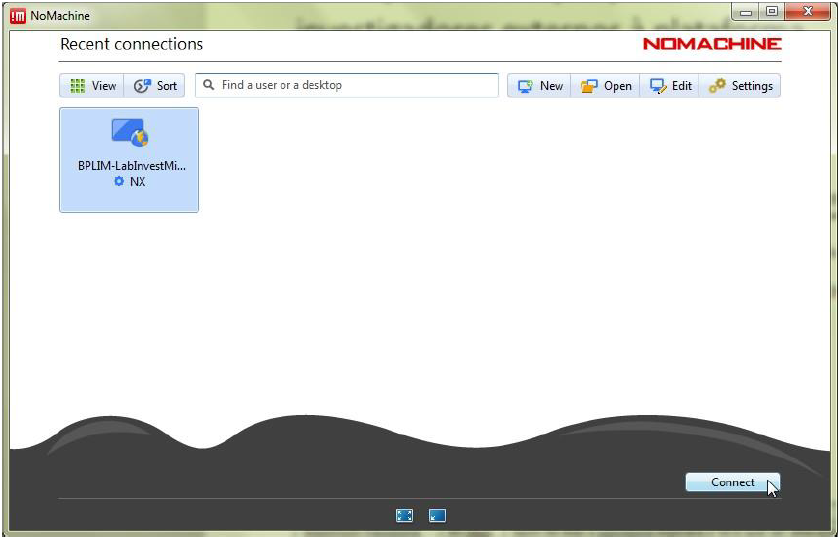
\includegraphics[width=4.72441in,height=3.03698in]{./media/image32.png}
\end{quote}

\textbf{\hfill\break
}

\begin{quote}
\textbf{Step 5.8}: Before the first effective connection, it may be
necessary to accept the certificate from bplimexterno.bportugal.pt

The Investigator should verify that the "fingerprint" (verification
code) is:

\textbf{SHA256 ED 1B D9 E2 C2 F8 C6 08 1A 53 5F 97 DA 71 77 D9 D2 EE 7A
5F 9C 35 87 B3 19 F4 7E A1 CB 2C 68 0B}

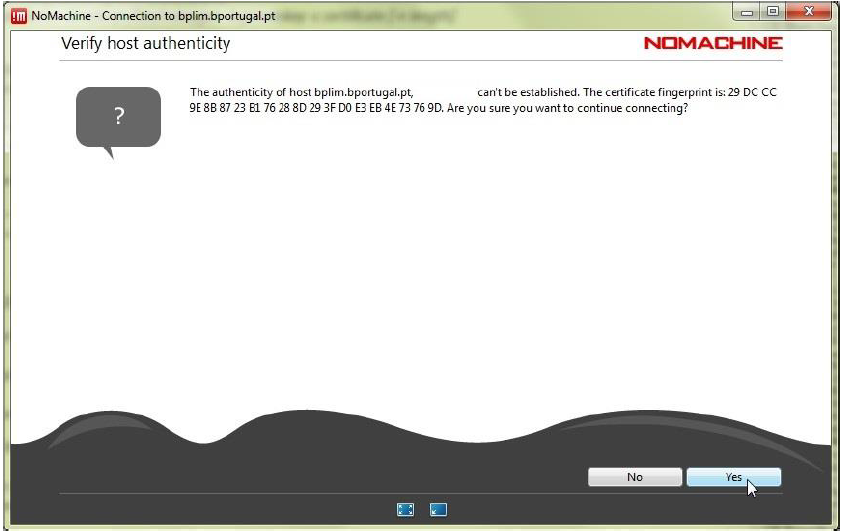
\includegraphics[width=4.72441in,height=2.98511in]{./media/image33.png}
\end{quote}

\textbf{\hfill\break
}

\begin{quote}
\textbf{Step 5.9}: Connect with the UserID (\textbf{case sensitive}) and
password provided by Banco de Portugal:

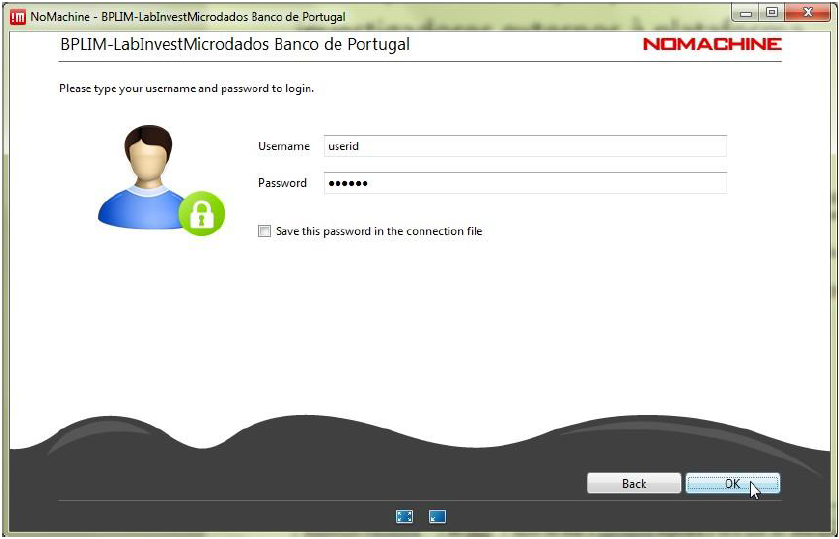
\includegraphics[width=4.72441in,height=3.03504in]{./media/image34.png}

\textbf{Step 5.10}: After the first successful login, it is necessary to
change the password, which must comply with the Password Policy defined
above.

If the new password does not comply with the Password Policy, the
original password provided by the Banco de Portugal will be
re-requested. See Appendix 3 for details.

The NoMachine client does not tell you why the new password was not
accepted -- it is the responsibility of the user to verify that the new
password is in compliance.

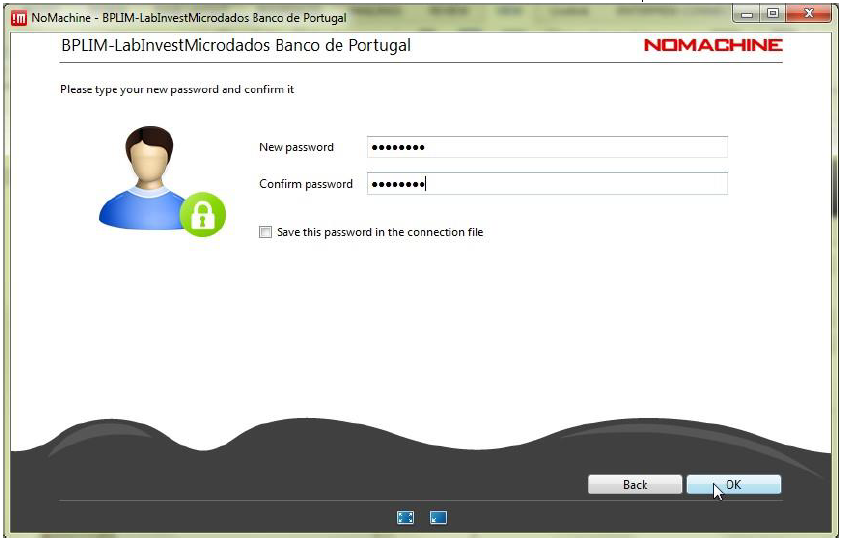
\includegraphics[width=4.72441in,height=3.02972in]{./media/image35.png}

\textbf{Step 5.11}: Upon login success, the following screens should
appear

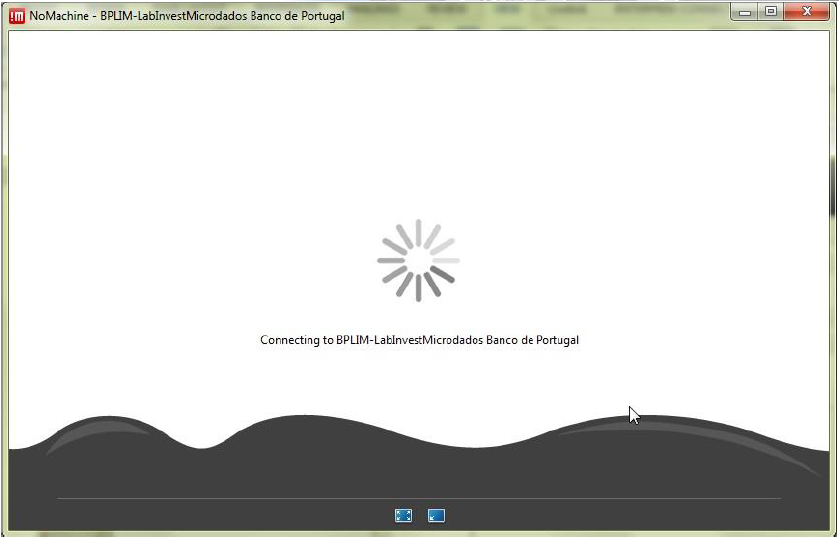
\includegraphics[width=4.72441in,height=3.02971in]{./media/image36.png}

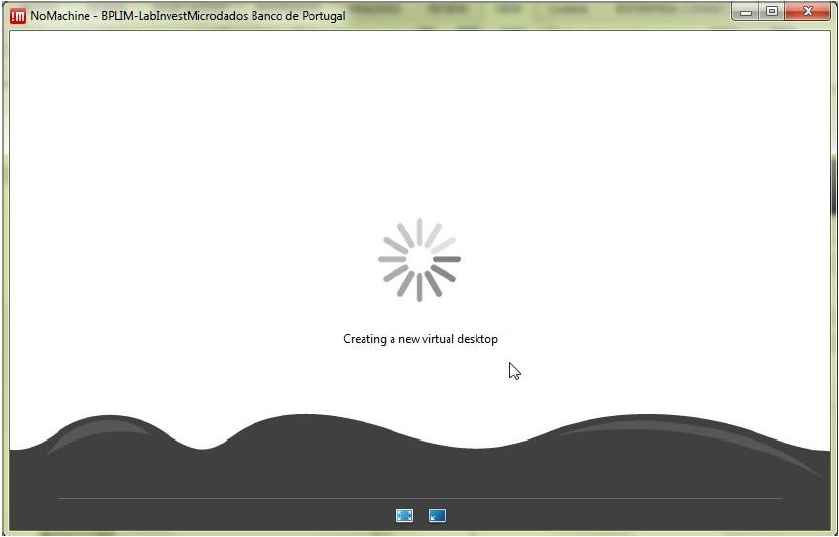
\includegraphics[width=4.72441in,height=3.02389in]{./media/image37.png}

Once logged in and with access to a KDE session, click on the upper
right corner of the KDE desktop, as shown below, to access the menu and
then expand the screen as exemplified for greater ease of use.

\textbf{Step 5.12}: You should see the following screen.

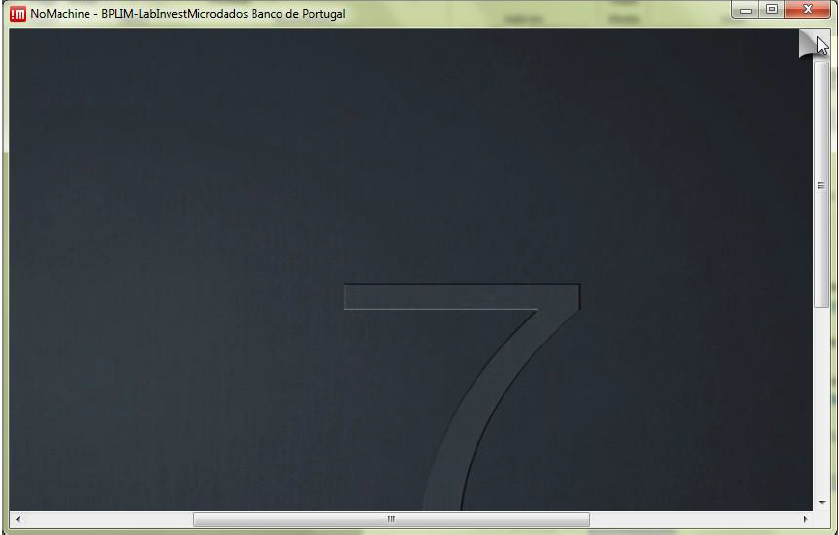
\includegraphics[width=4.72441in,height=3.01274in]{./media/image38.png}

\textbf{Step 5.13}: Click `Display'

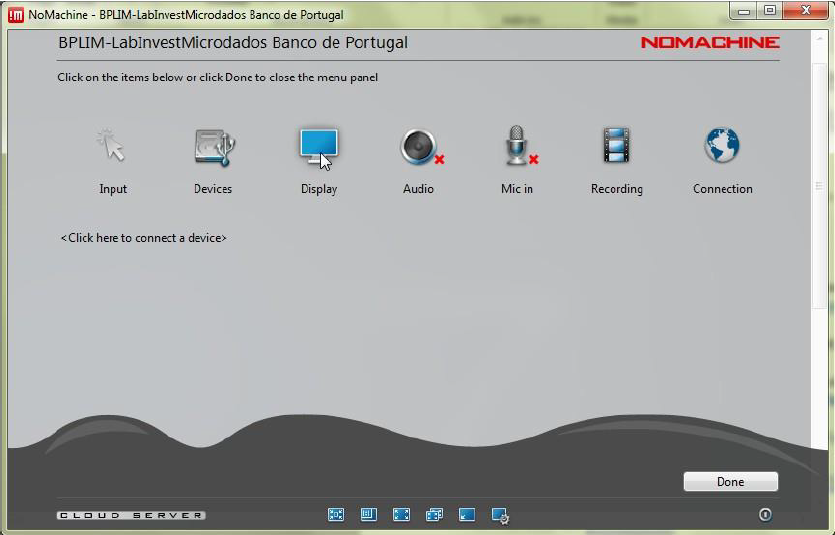
\includegraphics[width=4.72441in,height=3.0268in]{./media/image39.png}

\textbf{Step 5.14}: Click `Fit to window' and click `Done'

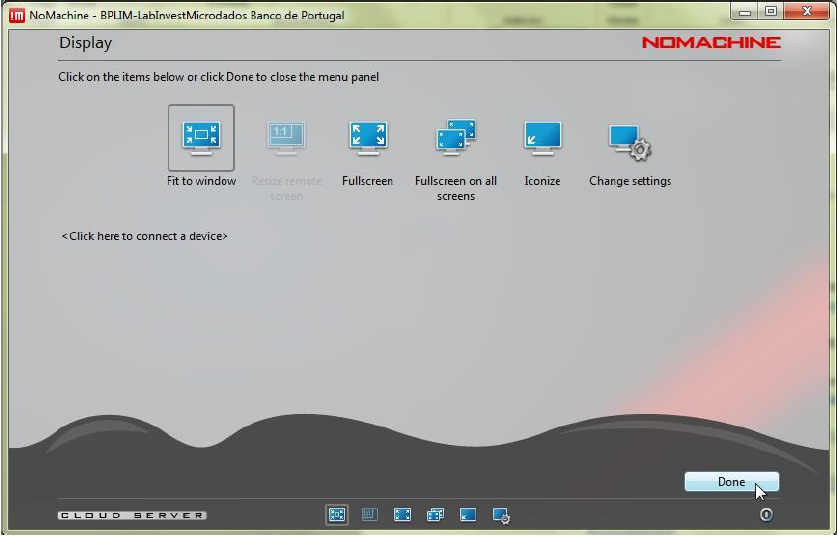
\includegraphics[width=4.72441in,height=3.02195in]{./media/image40.png}
\end{quote}

\hypertarget{frequently-asked-questions}{%
\subsection{Frequently Asked
Questions}\label{frequently-asked-questions}}

\begin{enumerate}
\def\labelenumi{\arabic{enumi}.}
\tightlist
\item
  Mac users are not able to install NoMachine, receiving the following
  message
\end{enumerate}

\begin{quote}
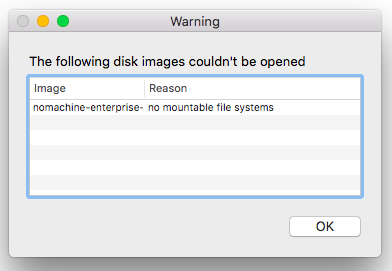
\includegraphics[width=2.16535in,height=1.49697in]{./media/image45.png}
\end{quote}

Please check if your Mac OSX is updated. Temporary solution: download
NoMachine Enterprise Client from the official website, and run the
installation file:

\url{https://www.nomachine.com/download-enterprise/\#NoMachine-Enterprise-Client}

\begin{enumerate}
\def\labelenumi{\arabic{enumi}.}
\setcounter{enumi}{1}
\tightlist
\item
  NoMachine authentication failure
\end{enumerate}

\begin{quote}
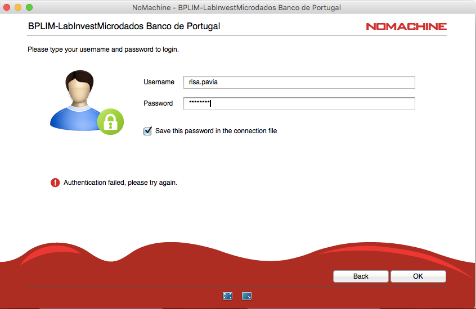
\includegraphics[width=2.16535in,height=1.40773in]{./media/image46.png}
\end{quote}

\begin{itemize}
\item
  In some cases, it occurs due to a different keyboard layout. For
  example, if you have a Portuguese keyboard, but the website assumes a
  US keyboard, and your password contains a symbol like `ç' then you
  will get a ``wrong password'' message. Please check the keyboard
  layout that is active when you type the password. Alternatively,
  change the password after the first login with NoMachine. Use linux's
  command `passwd'.
\item
  Login fails, and the system shows the message: "Could not connect to
  the server. Error is 138: Connection is timed out" Please check if
  your network has a strict firewall; e.g., some researchers are not
  able to reach BPLIM's server within their University network. Please
  check if in a different location, like at home, the connection works.
\end{itemize}

\begin{enumerate}
\def\labelenumi{\arabic{enumi}.}
\setcounter{enumi}{2}
\tightlist
\item
  User pressed `Lock' instead of `Log out' and the unlock/password does
  not work:
\end{enumerate}

\begin{itemize}
\item
  Check if the keyboard settings are correct (e.g., PT or UK)
\item
  Close the `NoMachine' connection and start a new one. Before the last
  step -before the \textquotesingle Login'- right-click and choose
  `Logout'. Double-click for the new connection
\end{itemize}

\begin{enumerate}
\def\labelenumi{\arabic{enumi}.}
\setcounter{enumi}{3}
\tightlist
\item
  ``Cannot see the screen in NoMachine'' (see image below)
\end{enumerate}

\begin{quote}
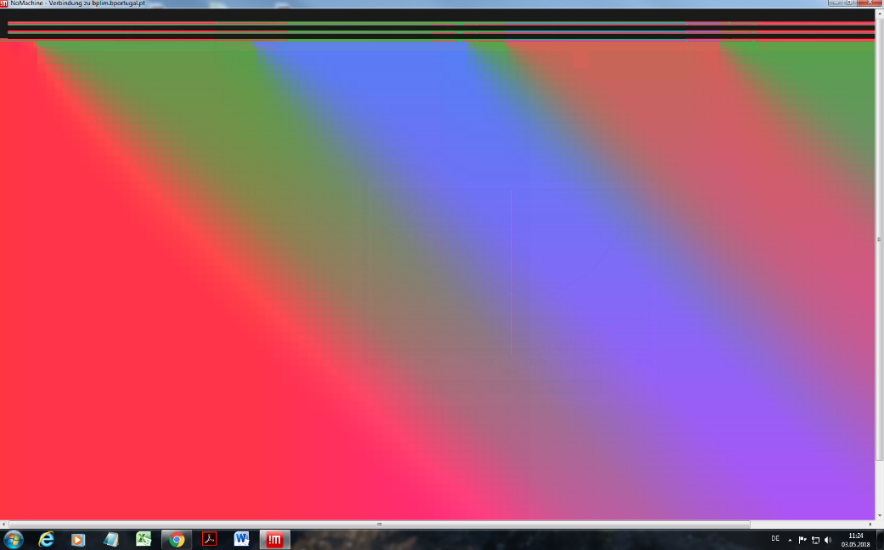
\includegraphics[width=4.01667in,height=2.49995in]{./media/image47.png}
\end{quote}

\begin{enumerate}
\def\labelenumi{\arabic{enumi}.}
\setcounter{enumi}{4}
\tightlist
\item
  \ul{OPTION A}: move your mouse on top the upper right corner of
  NoMachine, you should see a ``folded like sheet'', left-click your
  mouse, go to `Display', `Change settings', and click in `Disable
  client side hardware decoding'
\end{enumerate}


\includegraphics[width=1.56522in,height=0.15in]{./media/image48.png}

\begin{enumerate}
\def\labelenumi{\arabic{enumi}.}
\setcounter{enumi}{5}
\item
  \ul{OPTION B}: Close the `NoMachine' connection and start a new one.
  Before the last step -before the \textquotesingle Login'- right click
  and choose `Logout'. Double-click for the new connection
\item
  ``Error: Parameter `agentm\_display' has bad value'' (see image below)
\end{enumerate}

\begin{quote}
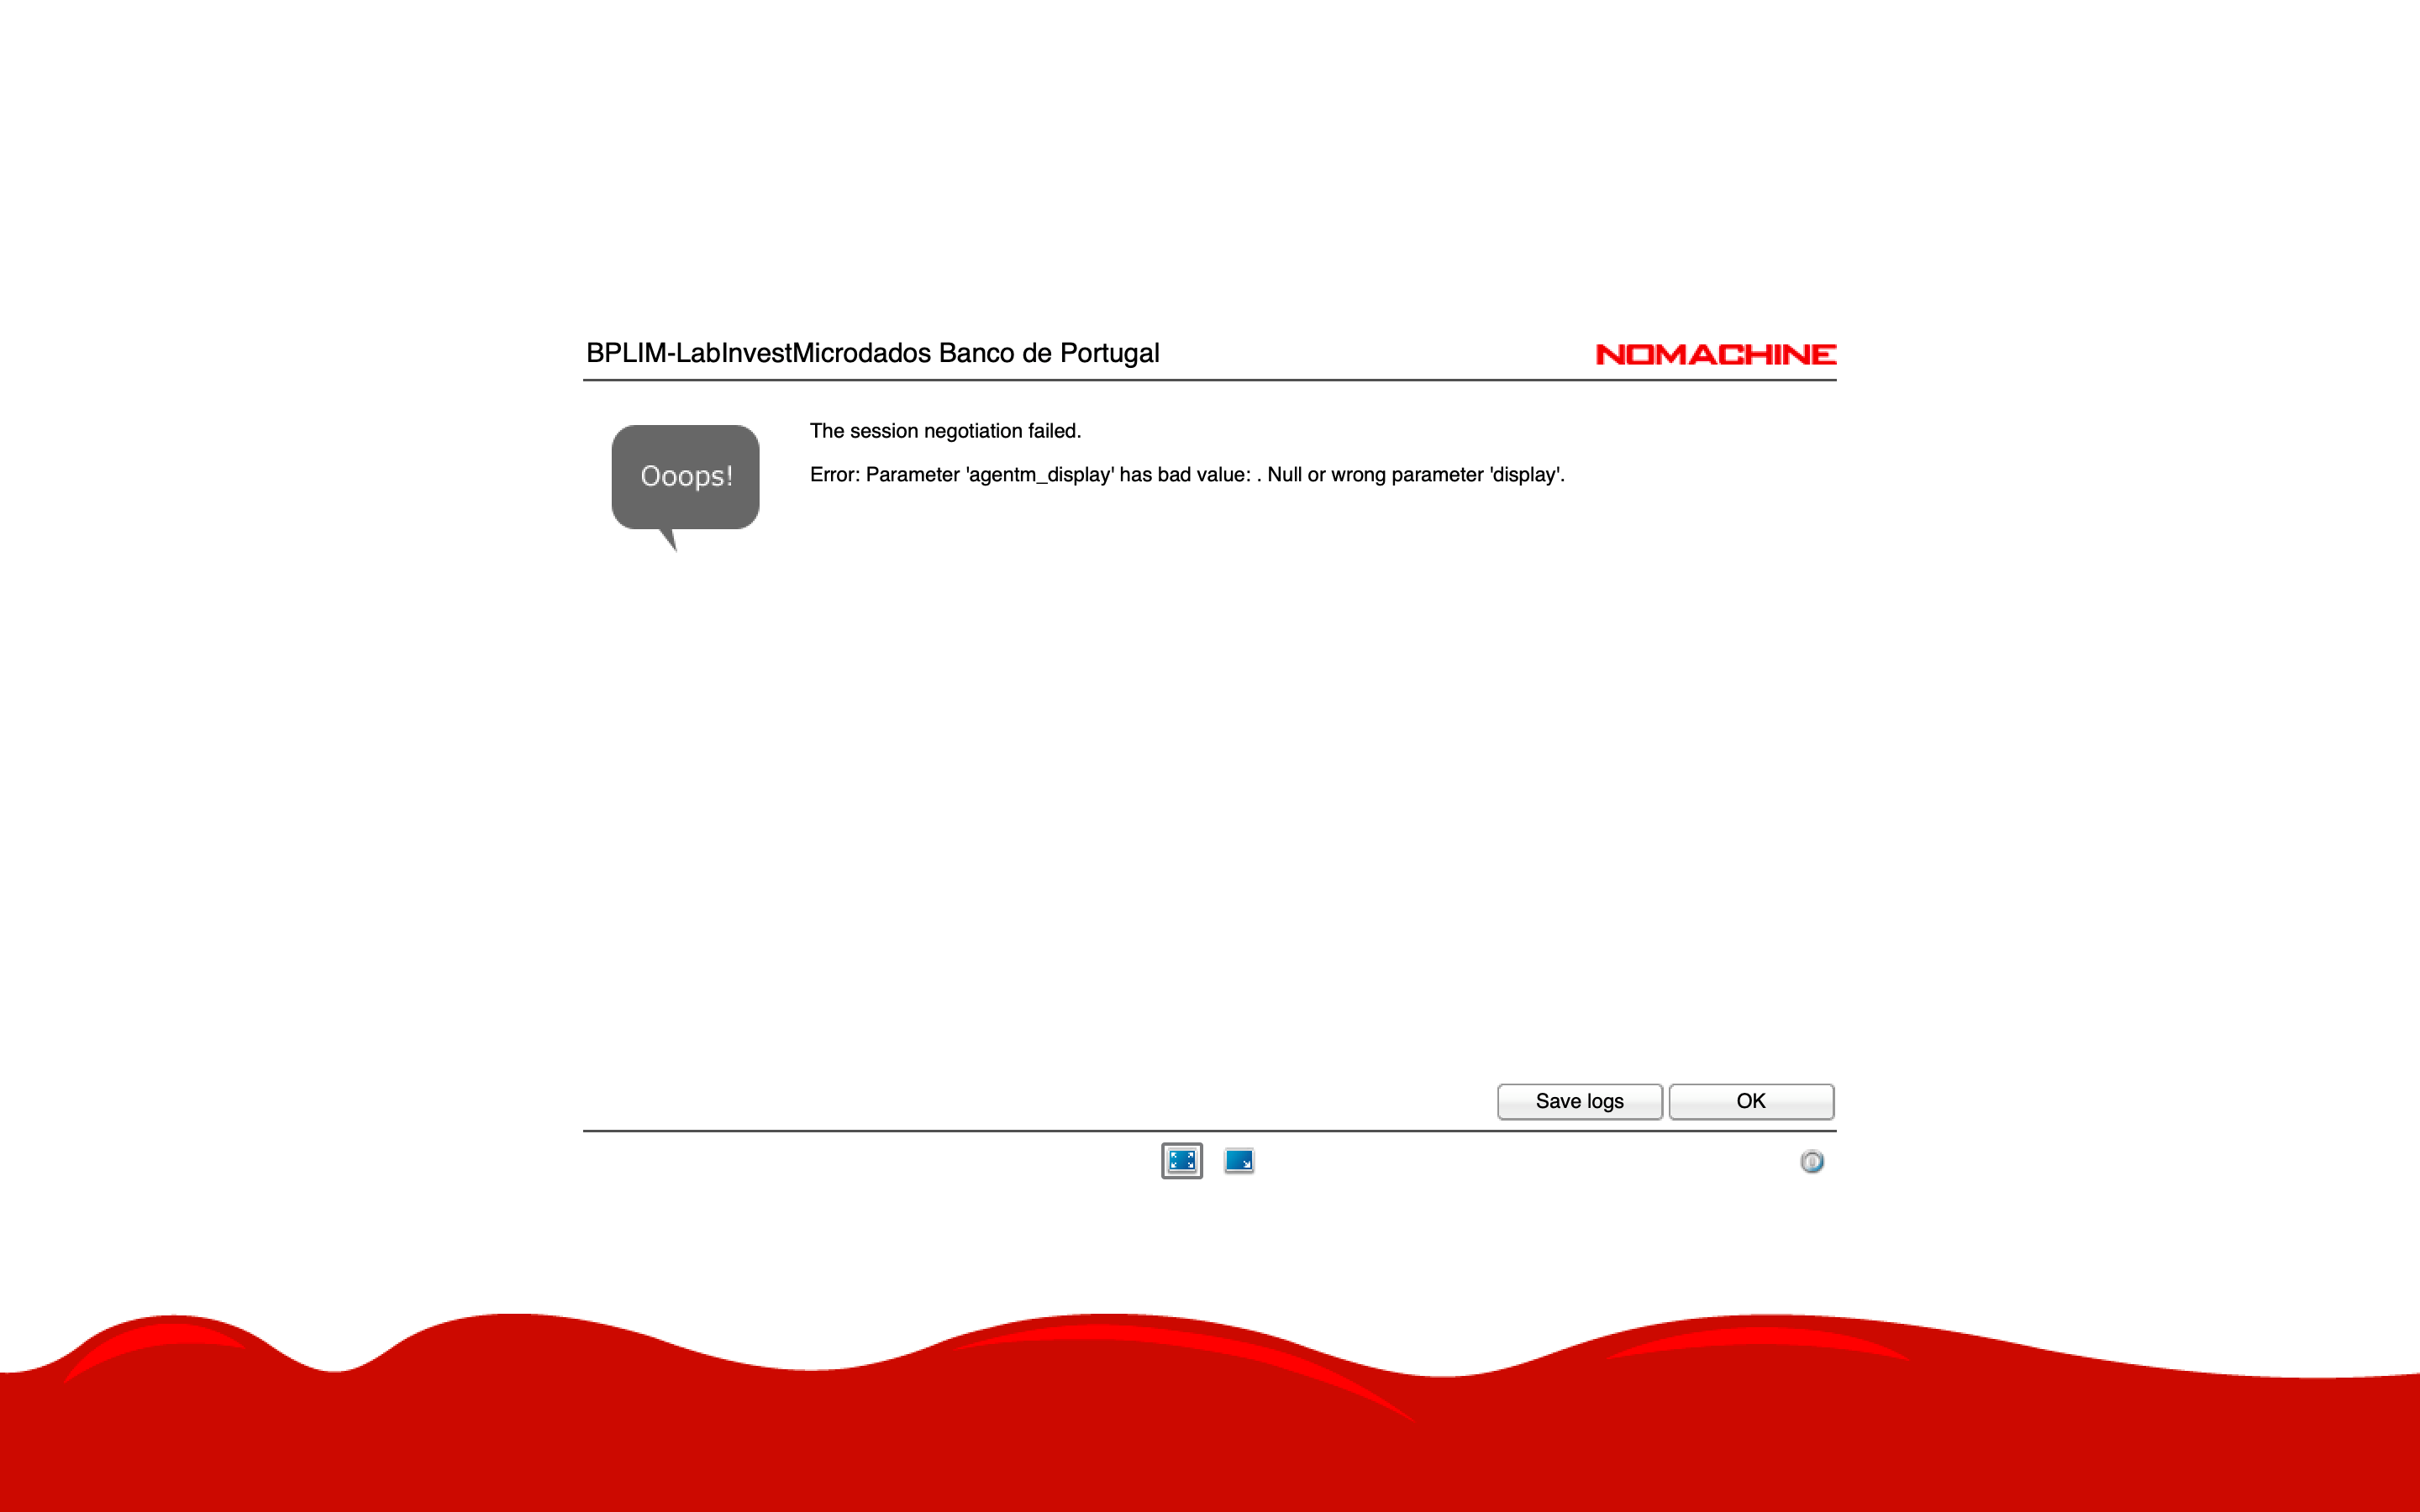
\includegraphics[width=4.01667in,height=2.49995in]{./media/parameter_bad_value.png}
\end{quote}

\begin{itemize}
\item
  Your home folder is full (/home/USER\_LOGIN): \textbf{\emph{Do not
  save files in your home folder}}
\item
  Ask BPLIM Staff to empty space in your home folder
\end{itemize}

\begin{enumerate}
\def\labelenumi{\arabic{enumi}.}
\setcounter{enumi}{7}
\tightlist
\item
  Session is frozen
\end{enumerate}

\begin{itemize}
\tightlist
\item
  Go to NoMachine first screen and double-click in the following icon
\end{itemize}

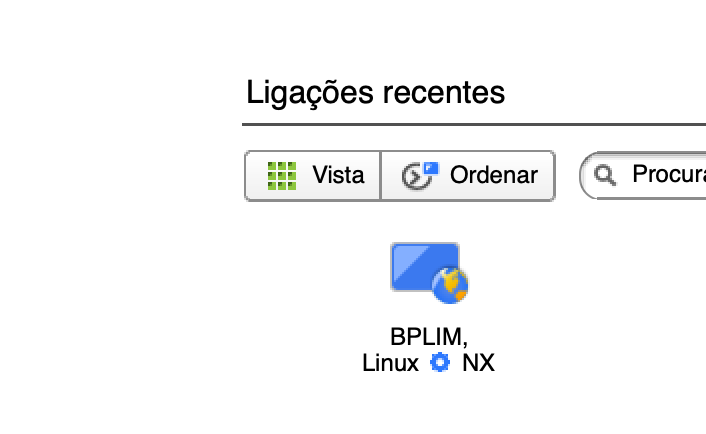
\includegraphics[width=3in,height=\textheight]{./media/logout1.png}

\begin{itemize}
\tightlist
\item
  right-click on the icon below and choose ``Terminar sessão''
\end{itemize}

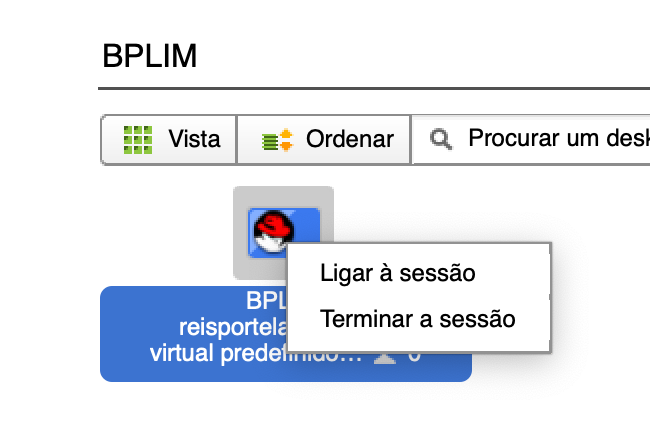
\includegraphics[width=3in,height=\textheight]{./media/logout2.png}

\begin{enumerate}
\def\labelenumi{\arabic{enumi}.}
\setcounter{enumi}{8}
\tightlist
\item
  Visualizing \LaTeX  tables
\end{enumerate}

\begin{itemize}
\tightlist
\item
  In case you want to see the pdf of tables you have exported to
  \LaTeX  you can create a generic tex file, \texttt{main.tex}, with the
  following content:
\end{itemize}

\begin{quote}
\texttt{\textbackslash{}documentclass\{article\}}

\texttt{\textbackslash{}begin\{document\}}

\texttt{\textbackslash{}input\{your\_table.tex\}}

\texttt{\textbackslash{}end\{document\}}
\end{quote}

\begin{quote}
where your table is `your\_table.tex'. The tex file can be compiled in
the Terminal by typing \texttt{pdflatex\ main.tex}.
\end{quote}

\hypertarget{version-control}{%
\subsection{Version control}\label{version-control}}

The server runs \href{https://git-scm.com/}{Git} version 1.8.3.1.

\begin{quote}
\href{https://en.wikipedia.org/wiki/Git}{Wikipedia}:

``Git is a distributed version-control system for tracking changes in
any set of files, originally designed for coordinating work among
programmers cooperating on source code during software development. Its
goals include speed, data integrity, and support for distributed,
non-linear workflows'\,'
\end{quote}

First steps

\begin{enumerate}
\def\labelenumi{\arabic{enumi}.}
\tightlist
\item
  move to a specific folder; \emph{e.g.},
  \texttt{cd\ /bplimext/projects/your\_project\_ID/work\_area/}
\item
  create a .gitignore file (check
  \href{https://www.toptal.com/developers/gitignore}{toptal} for some
  examples)
\item
  \texttt{git\ init}
\item
  \texttt{git\ add\ *.do}
\item
  \texttt{git\ commit\ -a\ -m\ "First"}
\item
  \texttt{git\ show\ first\_do\_file.do}
\end{enumerate}

\hypertarget{containers}{%
\subsection{Containers}\label{containers}}

\hypertarget{build-your-container}{%
\subsubsection{Build your container}\label{build-your-container}}

\begin{itemize}
\tightlist
\item
  You can write a script to build your container using our definition
  file template available at our
  \href{https://github.com/BPLIM/Manuals/tree/master/ExternalServer}{GitHub
  repository}:
\end{itemize}

\begin{quote}
\href{https://github.com/BPLIM/Manuals/tree/master/ExternalServer/Containers/1.R_RStudio/BPLIM_container_PROJECT_ID.def}{BPLIM\_container\_PROJECT\_ID.def}
\end{quote}

\begin{itemize}
\item
  In this template we setup a machine running Ubuntu 20.04, R 4.2 and
  RStudio.
\item
  You can add your packages in line 89 within \texttt{c()}; e.g.,
\end{itemize}

\begin{quote}
\texttt{c("tidyverse","haven")}
\end{quote}

\begin{itemize}
\item
  Test your script and build the container using
  \href{https://cloud.sylabs.io/}{SylabsCloud} (you can use your GitHub
  account to login)
\item
  Click in `CREATE'
\end{itemize}


\includegraphics[width=1.2in,height=\textheight]{media/SylabsCreate.png}

\begin{itemize}
\tightlist
\item
  In the following step upload your `.def' file or copy/paste its
  contents in the Text box:
\end{itemize}

\includegraphics[width=1.7in,height=\textheight]{media/SylabsBuildContainer.png}

\begin{itemize}
\item
  Sylabs runs a first test on the validity of your script and releases
  the button `Build' (click on it)
\item
  Follow the outcome at the bottom of the screen and check for possible
  error messages
\item
  Once you succeed in building the container, you can send us the
  definition file with your changes
\end{itemize}

\hypertarget{use-the-container-in-bplims-server}{%
\subsubsection{Use the container in BPLIM's
server}\label{use-the-container-in-bplims-server}}

\begin{itemize}
\item
  Open a \texttt{Terminal}
\item
  Move to your project's folder
\end{itemize}

\begin{quote}
\texttt{cd\ /bplimext/projects/YOURPROJECTID/tools/containers}
\end{quote}

\begin{itemize}
\tightlist
\item
  Start the container by typing
\end{itemize}

\begin{quote}
\texttt{singularity\ shell\ YOURPROJECTID.sif}
\end{quote}

\begin{itemize}
\item
  The prompt of the \texttt{Terminal} will show: \texttt{Singularity}
\item
  Start RStudio by typping \texttt{rstudio} (small caps)
\end{itemize}

\includegraphics[width=1.7in,height=\textheight]{media/Singularity_Terminal_Prompt.png}

\begin{itemize}
\tightlist
\item
  Once inside RStudio you have access to the original folder structure
  of your project
\end{itemize}

\hypertarget{jupyter-lab}{%
\subsection{Jupyter Lab}\label{jupyter-lab}}

Explore \href{https://jupyter.org/}{Jupyter lab}:

\begin{quote}
``JupyterLab is a web-based interactive development environment for
Jupyter notebooks, code, and data. JupyterLab is flexible: configure and
arrange the user interface to support a wide range of workflows in data
science, scientific computing, and machine learning. JupyterLab is
extensible and modular: write plugins that add new components and
integrate with existing ones.''
\end{quote}

Start Jupyter Lab by typing:

\begin{quote}
\texttt{jupyter\ lab}
\end{quote}

Sample session:

\includegraphics[width=0.65\textwidth,height=\textheight]{./media/JupyterLab.png}

\end{document}
